%TODO
%update tables
%reread text


%\documentclass[10pt,iop]{emulateapj}
\documentclass[preprint]{aastex}
%\usepackage{rotating}
\usepackage{url}
\usepackage{multirow}
\usepackage{amsmath}
%\usepackage{graphicx}
%\usepackage[figuresright]{rotating}
%\usepackage{rotating}
%%\usepackage{natbib}

%\citestyle{aa}

%\bibliographystyle{apj_w_etal}

\newcommand{\etal}{{et al.\/}}
\newcommand{\Prob}{\mathtt{P}}
\newcommand{\logL}{\log\mathcal{L}}
\newcommand{\unit}[1]{\footnotesize #1}
\newcommand{\PAPER}{\mathrm{PAPER}}
\bibliographystyle{apj_w_etal}

	% End definitions

%\slugcomment{DRAFT: \today}

\shorttitle{Southern Hemisphere Flux Scale}
\shortauthors{Jacobs et al.}

\begin{document}

%\title{The Reionization flux scale in the Southern Sky}
\title{A Flux Scale for Southern Hemisphere 21cm EoR Experiments}
\author{
Daniel C. Jacobs\altaffilmark{1},
Aaron R. Parsons\altaffilmark{2},
James E. Aguirre\altaffilmark{3},
Zaki Ali\altaffilmark{2},
Richard F. Bradley\altaffilmark{4,5,6},
Chris L.  Carilli\altaffilmark{7},
David R. DeBoer\altaffilmark{8},
Matthew R. Dexter\altaffilmark{8},
Nicole E. Gugliucci\altaffilmark{5},
Pat Klima\altaffilmark{5},
Dave H. E. MacMahon\altaffilmark{8}
Jason R. Manley\altaffilmark{9},
David F. Moore\altaffilmark{3},
Jonathan C. Pober\altaffilmark{2},
Irina I. Stefan\altaffilmark{10},
William P. Walbrugh\altaffilmark{9}}

\altaffiltext{1}{School of Earth and Space Exploration, Arizona State U., Tempe, AZ}
\altaffiltext{2}{Astronomy Dept., U. California, Berkeley, CA}
\altaffiltext{3}{Dept. of Physics and Astronomy, U. Pennsylvania, Philadelphia, PA}
\altaffiltext{4}{Dept. of Electrical and Computer Engineering, U. Virginia, Charlottesville, VA}
\altaffiltext{5}{National Radio Astronomy Obs., Charlottesville, VA}
\altaffiltext{6}{Dept. of Astronomy, U. Virginia, Charlottesville, VA}
\altaffiltext{7}{National Radio Astronomy Obs., Socorro, NM}
\altaffiltext{8}{Radio Astronomy Lab., U. California, Berkeley, CA}
\altaffiltext{9}{Square Kilometer Array, South Africa Project, Cape Town, South Africa}
\altaffiltext{10}{Cavendish Lab., Cambridge, UK}

\begin{abstract}
We present a catalog of broad-band spectral measurements from the 
Donald C. Backer Precision Array for Probing
% XXX ARP: was irina "first"?  and maybe "catalog"
the Epoch of Reionization (PAPER) in South Africa observed in July and
September of 2011.  In order to reduce the impact of beam calibration, which proves to
be a difficult endeavor for transit telescopes such as PAPER, on the determination
of source spectra, we have focused on calibrating sources in a narrow declination range.
Since each source follows a nearly identical path through the primary beam, this
restriction allows beam calibration to be nearly eliminated as a source of error,
yielding a dramatic improvement in the accuracy of source spectra measured in the 
100--200-MHz band that is receiving renewed attention by experiments seeking to
measure 21cm emission from the Epoch of Reionization (EoR).
Based on the variation in our data and the estimated error in the absolute
flux scale we bootstrap from multiple bright sources, we estimate PAPER measurements
of sources above XXX Jy to be accurate to 3.2\%.
% DCJ 3.2% is just for Pictor A, and certainly not all PAPER measurements of sources above XXX Jy
When combined with catalog data at other frequencies, these data constrain parameters of
a power-law model for flux density with an uncertainty of 2.4\%.
% XXX ARP: this must again be dependent on source strength and location.
This accuracy is limited by the uncertainty in the catalog measurements we use
to estimate an absolute flux scale, and represents 
an order of magnitude improvement over previous measurements in this band.  
Comparing with prior measurements, 45 out
of 58 sources observed are found to confirm and refine a power-law model for flux density.
This includes Pictor A, which provides a key flux reference for PAPER's EoR
power spectrum analysis.
\end{abstract}

\keywords{dark ages, reionization, first stars --- catalogs --- instrumentation: interferometers}

% XXX remove references to appendix

\section{Introduction}

Numerous radio telescopes are now exploring the prospects for using
measurements of highly redshifted 21cm emission to inform our understanding of
cosmic reionization in the redshift range $6< z<12$, corresponding to radio
frequencies below 200 MHz (see reviews in
\citealt{Furlanetto:2006p2267,Morales:2010p8093,Pritchard:2012p9555}).  These
include telescopes aiming to measure the global temperature change of 21cm
emission during the Epoch of Reionization (EoR), such as the Compact
Reionization Experiment (CoRE) and the Experiment to Detect the Global EoR
Signature (EDGES; \citealt{Bowman:2010p8546}), and interferometers aiming to
measure the power spectrum of 21-cm EoR emission, such as the Giant Metre-wave
Radio Telescope (GMRT;
\citealt{Paciga:2011p9470,Paciga:2013p9627})\footnote{\url{http://gmrt.ncra.tifr.res.in/}},
the LOw Frequency ARray (LOFAR;
\citealt{Yatawatta:2013p9699})\footnote{\url{http://www.lofar.org/}}, the
Murchison Widefield Array (MWA;  \citealt{Bowman:2012p9138};
\citealt{Tingay:2013p9022}))\footnote{\url{http://www.mwatelescope.org/}}, and
the Donald C. Backer Precision Array for Probing the Epoch of Reionization
(PAPER; \citealt{Parsons:2010p6757,Parsons2013b})\footnote{\url{http://eor.berkeley.edu/}}.

As such, there has been a renewed interest in the spectral and spatial variation of
foreground emission in the 100--200 MHz frequency band that covers
the $z=6$--13 redshift range expected to encompass reionization
\citep{furlanetto_et_al2006}.
In particular, the spectral properties of extra-galactic point-sources are important
both because they are valuable calibration references
and because they are strong foreground emitters that must be removed from 21-cm EoR measurements.
With the sparse availability of measured foreground properties in the
100--200-MHz frequency band over large areas of the sky \citep{deolivieracosta_et_al2008}, continued
foreground characterization is a
vital step en route to any 21-cm EoR detection.
At these low
frequencies the Southern sky is much less well known than the North, 
with catalog source fluxes at 150MHz being inaccurate at the 20\% level
for $\delta<-20$\arcdeg (XXX cite).
Both PAPER and the MWA are located in the southern hemisphere at radio-quiet
reserves being prepared for the upcoming Square Kilometer Array, and hence,
the
most extensive surveying work is now being conducted by the EoR experiments
themselves \citep{Jacobs:2011p8438,Williams:2012p8768}.

One significant complication to improving the state of affairs in foreground characterization
is that many 21cm EoR experiments, including LOFAR in the northern hemisphere, and
PAPER and MWA in the southern hemisphere, are designed for drift-scan observations.
This design decision has largely been driven by the simplicity and cost-effectiveness of
phased and/or correlated dipoles for achieving the aggressive sensitivity requirements
for measuring the 21cm power spectrum of reionization (XXX cite).
Adding to the challenge, these telescopes 
cover much wider fields of view ($>10$\arcdeg) and bandwidths
($\sim 100$\% fractional) than traditional dish telescopes.
Because they do not physically point, flux calibration for such arrays relies heavily
on an accurate model of the primary beam response to correct for an
the apparent flux scale that varies across the sky.
This direction dependent gain is currently uncertain to 10\% or higher
% XXX 20% seems a bit grim.  Doesn't jonnie argue for 5 to 10% in his paper?
%XXX 20\% comes from the overall uncertainty between MWA and PAPER, part of which is also side lobes. 
%	Jonnie's fluxes are dominated by the side lobes in the pgb16 data, the fluxes have a range of errors around 15 to 20%
\citep{Pober:2012p8800}, and comprises a large fraction of the 20\% difference between current telescopes \citep{Jacobs:2013p9713}.

In this paper, we set out to significantly improve the accuracy of spectral measurements between 
100--200 MHz for a set of bright sources in the declination range XXX to XXX that
are of particular value for southern-hemisphere 21cm EoR experiments such as PAPER and the MWA.
Using the fact that, for this restricted declination range,
sources transit through a nearly identical primary beam response pattern, we are able to avoid one of the
most debilitating source of error in these measurements: the primary beam.  
% XXX update document map
In \S\ref{sec:analysis} we describe our approach for measuring source spectra with
drift-scan observations and deriving an absolute flux scale from catalog data.  
In \S\ref{sec:Observations} we detail the instrumental 
setup, observations and analysis method followed. In \S\ref{sec:fits} we
compare the spectra with available data.  We conclude in 
\S\ref{sec:Conclusion}.


%The ideal solution is to use a wide-grid of
%well-known calibrators to map the primary beam and set the flux scale.  
% XXX don't go to "ideal solution" just yet
% XXX ARP: add importance of accurate flux vs. frequency (Parsons et al. 2012, etc.)

%The position dependent gain varies for each instrument.   LOFAR and MWA have a range of electrically steerable beams each with a different shape. For MWA and LOFAR, the number of high quality calibration sources is more important.  PAPER has a single broad, 45\arcdeg wide, primary beam; sources at nearby declinations sample the same primary beam many times.
% This will in turn provide a wide base to assess the accuracy of the primary calibrator which sets the overall amplitude of the EoR power spectrum.  

\section{Background}

% XXX unsure about this section.  need someplace to give overviews of catalogs

Historically, the best
EoR band data were by \citet{Slee:1995p7541} with Culgoora Circular
Array\footnote{Known during daylight hours as Culgoora Radio Heliograph} and
various higher frequency measurements with Parkes.  These data are typically
uncertain to 20\% or higher and provide little coverage of the EoR band beyond
a single narrow-band data point. 

More recent surveys include narrow-band surveys by the GMRT and Mauritius, a
deep survey of the region near Hydra A by the 32 antenna MWA prototype
\cite{Williams:2012p8768} and a wide field survey by PAPER, also with 32
elements \cite{Jacobs:2011p8438}. Several sub-channels were provided in the
Williams catalog, though with 60-80\% error bars ---large compared to the 30\%
uncertainty on their wide band measurements.  The latter cover the band and
spatial scales relevant to EoR measurements but are limited by the accuracy of
the primary beam \citep{Jacobs:2013p9713}.

A method for decoupling uncertain fluxes from the uncertain beam has been
described by \citet{Pober:2012p8800}. In simulation the method was able to
achieve 3 to 10\% accuracy in measuring the primary beam, depending on the
number of antennae and other variables. The Pober method emphasized the need
for many repeated measurements of each alt-az pointing. Further investigation
is under way to improve and implement this method and would be greatly aided by
the availability of precise flux measurements unaffected by primary beam
uncertainty. 

This paper reports a set of flux measurements where a primary beam
model has not been used to estimate the flux, but instead are directly
calibrated to a single calibrator making the track through the beam.


EoR measurements in the southern sky have focused on the coldest regions where
galactic foregrounds are minimal. With the majority of possible observing time falling on 
RA=4h,Dec=-30. The brightest and least-resolved calibrator in this region is Pictor A 
(5h19m49.1 -45d46m45.0). Pictor A is a nearby FR-II type radio galaxy 
 similar to Cygnus A.  At $\sim$400Jy Pictor is bright and sufficiently distant from other 
bright sources to make it eminently suitable as both a phase and flux calibrator. Its apparent
size of $\sim$8\arcmin is smaller than the scales being probed by current EoR instruments , 
making resolution effects, making it suitable for precision calibration.  However, 
like most other sources, precise flux measurements in the EoR band are not available.
The current best EoR band measurement
is uncertain to 12\% and appears to imply spectral flattening in the EoR band
\citep{Perley:1997p9312}. 
 
%0518-458	 PKS, Pictor A	G	 25.93	 24.01	1		W	 0.0342	 23.63	 176.
% XXX transition to the PAPER instrument
Establishing an accurate spectrum for Pictor A is of particular importance for
PAPER --- a dedicated EoR experiment 
that employs drift-scanning, dual-polarization dipole antennas 
tuned for efficient operation over a 120--170-MHz band.  PAPER is located in the South African Karoo desert
on the Square Kilometer Array
South Africa (SKA-SA) reserve, 100km north of the small town of Carnarvon.
The PAPER array has grown from 16 elements deployed in early 2009 to a
64-element imaging array in 2011 (see Figure \ref{fig:antpos}). 
Since November 2011 it has been arranged in a maximally redundant grid 
configuration to make deep power spectral integrations \citep{Parsons:2012a}.
Though highly sensitive as a power spectrum instrument, the maximally redundant array 
has a broad point spread function in the image domain. This severely limits the number 
of sources which may be used for flux calibration. Drift scanning across the sky with a 45\arcdeg FWHM
primary beam there are very few unresolved, bright sources which are far from the galactic plane. 
Pictor A is bright and well enough separated from other emission to dominate the visibilities for a good fraction of
the EoR observing season, making it an ideal flux calibrator.





\section{Approach}
\label{sec:approach}
Given the large uncertainties in the literature, and the necessity for PAPER power-spectrum analysis
to use Pictor A for flux calibration, we felt it prudent to examine Pictor A directly.
In this section, we describe how we use PAPER in its imaging configuration
to measure Pictor A and a selection of known, bright sources in a 5\arcdeg strip centered
on -45\arcdeg. 

 In \citet{Jacobs:2013p9837} several limitations were identified that
exasperated the primary beam uncertainty.  First, in imaging each source flux is measured at just a few 
points in the primary beam. As errors tend to vary across the beam, the uncertainty will tend to vary between sources.
Here we have averaged over all possible positions making the uncertainty a function of the net uncertainty in the beam,
and stabilizing the source-to-source variations in error bars. The second limitation, identified in \citet{Williams:2012p8768},
was the increase of uncertainty towards the edge of the beam. To minimize our sensitivity to both beam and noise
uncertainty, we weight the source track by an additional factor of the primary beam model.  


As PAPER is a drift scan instrument, each declination $\delta$ describes a distinct cut through the primary beam. These cuts
provide a detailed measurement of the primary beam relative to the peak of the trace, however,
a model $g(\delta)$ is still required to calibrate between declinations. This model will be effective over a range of declinations, but will diverge at
some rate depending on the accuracy with which the model describes the slope.  As an estimate of the extrapolated 
beam amplitude we fit the slope of our Pictor A source track and compute the amplitude extrapolated over our fiducial
stripe width of 5\arcdeg.

\[
B = dB/dt dt/\theta \Delta \theta
\]

Comparing this with the simulation in Figure \ref{fig:beam_extrapolation}, we find that the model predicts the 5\arcdeg extrapolation to better
than 2\% even into the more uncertain areas far from zenith. The RMS difference for the central 15\arcdeg of the track
is 1.5\%. From this we conclude that, as long as we constrain our extrapolations to $\pm5$\arcdeg around Pictor A,
we will have negligible beam area. 

\begin{figure*}
\includegraphics[width=.9\textwidth]{plots/beam_slope_compare.png}
\caption{The beam is well along a declination cut but beam formed source tracks. Here we measure the beam, 
as extrapolated by fitting a slope (dotted), and compare with the beam model (solid). The difference (circles) is never larger
than $\sim$1\%.  Thus we conclude that the beam slope is locally well modeled and our beam model is suitable 
for extrapolation over $\sim$5\arcdeg scales.
  \label{fig:beam_extrapolation}}
\end{figure*}

We choose sources from the Molonglo
Reference Catalog \cite[MRC]{Large:1981p7798} that are within 5\arcdeg in
declination of a common calibrator (J2331-416) and have a flux extrapolated
from 408MHz greater than 10Jy assuming a power law spectral index of
-1.\footnote{Most radio sources in this band have power law spectra $S(\nu) =
\left(\frac{\nu}{\nu_0}\right)^\alpha$. } This selection contains 62 sources in a narrow
stripe that passes through the majority of the southern EoR fields, much of the
galaxy and Centaurus A. This stripe in the broader context of the galactic plane
is shown in Figure \ref{fig:error_map}.
A list of these 
sources is given in Table \ref{tab:src_spec}. 

For these sources, spectral data measured below 2 GHz were compiled from 
the NASA/IPAC Extragalactic Database (NED)
\footnote{\url{http://ned.ipac.caltech.edu/}}. Cross-matching radio sources
between bands is made difficult by changes in resolution, spectral curvature,
and resolved multi-scale structure.  For a small number of sources these
problems can be ameliorated by inspection of the spectra, source names,
coordinates,  and originating publications. However for a large sample of
sources this becomes unwieldily and prone to error. Thus for the larger number
of samples we make use of the Vollmer et al meta-catalog which takes pains to
match multi-wavelength observations \citep{Vollmer:2010p6422}.
% given the known source dimensions and spectral properties as well as telescope bandwidth and spatial resolutions. 

The spectra reported here are measured by beam-forming, phasing the visibilities to
the target location, and summing to produce a dynamic spectrum. The spectrum is then isolated
from neighboring sources by filtering and averaged in the time domain.  This time average is 
weighted by an additional factor of the PAPER's primary beam response 
\citep{pober_et_al2012}.  
\begin{align}
S_\textrm{est} &= \frac{\sum_t B_M S_p}{\sum_t B^2_M}\\
&= \frac{\sum_t B_M B}{\sum_t B^2_M} S\\ \label{eq:g}
\end{align}

which is an effective approximation of inverse-variance weighting. The pre factor in Eq \ref{eq:g} is identical for 
sources at the same declination, and as we found above, diverges slowly from the model in the 10\arcdeg declination stripe.
We estimate this spectral dependent gain for a calibrator (J2331-416) fitting a spectral index model to the
 well-defined data points below 2GHz. This removes an overall offset.
 
 Finally we average the spectra from a resolution of 400kHz to 10MHz bins, taking the standard deviation within these bins
 for an estimate of the uncertainty.

At this point we have a set of spectra that have been calibrated relative to each other to the best of our ability. Now 
they must be put on a global flux scale. We also have only a limited estimate of our error from our intra-channel
rms.  To address both points we fit for a global flux scale that incorporates data from many catalogs. These catalogs
have all been set, as best as possible, to the Baars et al scale.  Using a Bayesian analysis we compute the 
variation in the flux scale implied by comparing many sources to prior catalog. By including sources from across
the declination range,the variation in this flux scale fit estimates the overall uncertainty in flux resulting from primary beam 
or prior catalog uncertainty.  So though the final scale is calibrated to the Baars scale as extrapolated beyond its
defined band, the error on the flux scale fully encapsulates the error resulting from this extrapolation.

 
 \section{Data Reduction}
 \label{sec:Observations}

% XXX in this section, we describe the details of data analysis used ...
% XXX connect to Parsons2010,2013, pober2013, stefan2012, jacobs2011? for similar basic pipeline.

\begin{figure*}\centering
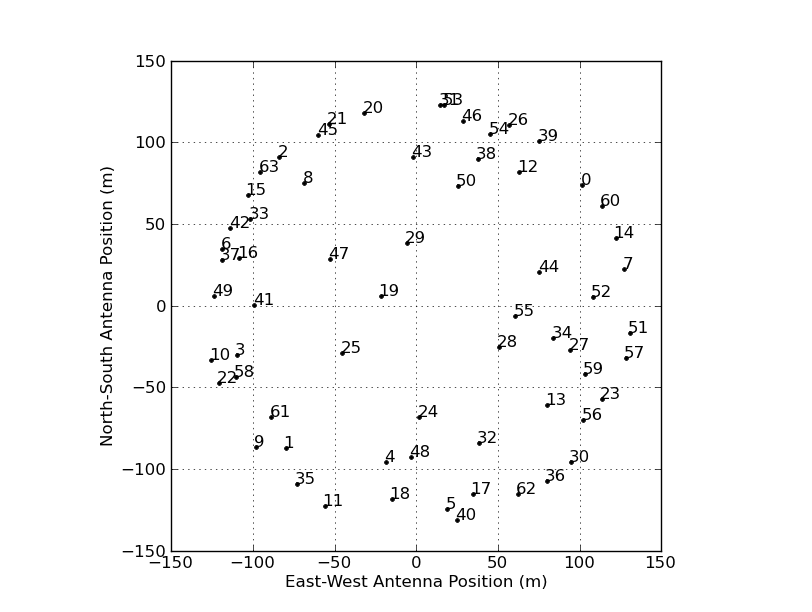
\includegraphics[width=0.85\columnwidth]{plots/antpos.png}
\caption{Antenna position in the 64-antenna, minimum-redundancy PAPER array configuration at the Karoo Radio Observatory site in South Africa used for these observations.
Data was captured during July and October of 2011 on a single 'x' polarization over a band between 120 and 180 MHz.
}\label{fig:antpos}
\end{figure*}

\subsection{Observations}

 Measurements are derived from observations using  the east-west dipole arms of
64 PAPER antennas deployed in a minimum-redundancy imaging configuration
(see Figure \ref{fig:antpos})
at the Karoo Radio Observatory site in South Africa.
A 100-MHz band from 100-200MHz was correlated
with 2048 frequency channels and integrated for 10.7 seconds before
visibilities were stored.  Observations included here on  July 4, 2011, running
from JD2455748.17 to JD2455748.72. and October 17, 2011 running from
JD2455852.2 to JD2455852.6.  In both seasons two antennas were omitted owing to
malfunctioning signal path. This 20 hour long combined dataset provides
observations provides complete hour angle coverage for the entire 24 hours of
Right Ascension. The July portion of the dataset comes from the same observing
campaign described by \cite{Pober:2013p9567} and \cite{Stefan:2012p9707}. 
%July (\#40,\#55), September (\#7,\#28) 

%COMPRESSION
\subsection{Data Compression}

In pre-processing, we use delay/delay-rate (DDR) filters
\citep{Parsons:2009p7859} to identify radio-frequency interference (RFI)
events, and as part of a data compression technique that reduces data volume by
over a factor of 40.  A more detailed description may be found in Appendix A of
\cite{Parsons2013b}, which uses the same compression method on PAPER power
spectrum observations. Here we summarize the process.

First, we remove known RFI transmission bands and analog filter edges, and then
flag outliers at 6$\sigma$ to remove RFI events.  Next, we suppress foreground
emission by applying a DDR filter to remove delays and delay-rates within the
horizon limit of a 300-m baseline (the maximum length of any PAPER baseline).
We derive a second set of RFI flags by masking 4$\sigma$ outliers in these
residuals and apply these flags back to the unfiltered data.  Finally, we
compress the data by applying a DDR filter preserving emission within the
horizon limit of a 300-m baseline, deconvolving to suppress flagging artifacts,
and down-sampling the result in time/frequency domain to the critical Nyquist
rate of the DDR filter.  The result is that the 2048 original frequency
channels become 203, and the 60 original time samples per 10-minute file become
14. 

% XXX merge with below
%Removed RFI by flagging samples in each frequency channel versus time that exceed the mean amplitude by 4-sigma
%after performing a time derivative.  Also flagged samples in each integrated spectrum that exceeded the
%mean amplitude across the spectrum by 6-sigma after performing a frequency derivative.  For efficiency, flagging
%was derived using only the subset of baselines involving a fiducial antenna.
%Frequencies below 120 MHz and above 180 MHz were also flagged, owing to roll-off of analog response.
%After RFI flagging, frequency channel resolution was decreased by a factor of four by summing channels.

%I'm Confused.  These are describing a different ordering of steps. Must re-read compression script.  

%CALIBRATION
\subsection{Per-Antenna Gain Calibration}

% XXX differentiate amp cal here from spectral cal and absolute cal that comes later.

Small gain variations between antennae and over time introduce significant systematic effects which degrade 
instrument performance. Temporal variations are dominated by changes in ambient temperature. 
Measurements of ambient temperature versus time near the balun amplifier of a fiducial antenna and near
receiver amplifiers were used to divide out the predicted gain variation versus temperature that these amplifiers
are known to exhibit.  A predicted gain profile was derived using coefficients characterized in
laboratory measurements \citep{parashare_bradley2009} and
confirmed in field measurements \citep{pober_et_al2011} of $H_{\rm balun}=-0.024$ dB/K, $H_{\rm recvr}=-0.045$
dB/K, and $H_{\rm cable}=-0.018$ dB/K for 150m-long cables.  Because cable temperatures were not measured
during these observations, the cable temperature was assumed to be the same as the measured balun temperature.


Matching of relative gains and phases between antenna was done by fitting a per-antenna complex gain to portions
of data which have easily modeled sky. 
This calibration is only relative between antennae, absolute flux calibration
comes after time and frequency averaging in  \S \ref{sec:flux_scale}.   
The antenna delays and amplitudes were found by fitting a point source visibility
model to Centaurus A, Pictor A, and Fornax A.  Each source is imperfectly
modeled by a single point-source, but the solution differences are minimized by
averaging over the three independent solutions. These same calibration
solutions have been successfully applied in \citet{Pober:2013XXX} and \citet{Stefan:2013:XXX}.
for power-spectrum analysis of foregrounds and imaging of Centaurus A, respectively.

% XXX incorporate
%To measure the spectrum of each source, we begin by applying per-antenna phase and gain
%calibrations established via self-calibration.  We next remove
%the known dependence of amplifier gain and cable attenuation on ambient temperature 
%using measured temperature data and temperature coefficients that were characterized in
%laboratory measurements \citep{parashare_bradley2009} and confirmed 
%in field-measurements \citep{pober_et_al2012}.  For each source, we phase to the source 
%osition
%and sum over 
%all baselines greater than 20 wavelengths in length.
%A fringe-rate filter (see \citet{parsons_backer2009} and Appendix A in \citet{Parsons2013b})
%is applied to the resulting
%beam to suppress beam sidelobes where sources introduce variations that deviate more than 
%$\pm$0.1 mHz from the fringe rate of the source in question.

%BEAMFORMING,FILTERING, AVERAGING

\subsection{Beamforming}

Spectral time-series are computed by beam-forming to the selected sky
locations. A beam is formed by phasing baselines to the desired location and
summing over baselines longer than 20 wavelengths.
%Samples were only included if there was a calibrator sample within 5\arcdeg in altitude/azimuth.   By using both seasons of data we were able to match all measurements with calibrator measurements, making this cut moot. 

% XXX incorporate paragraph below
%As the sky drifts through the primary beam of PAPER antennas, widely
%separated points will be observed with substantially different gains and
%so will require different data weightings to optimize SNR.
%Drift-scan observations of sources were divided by the calibrated beam response in the
%direction of the source as a function of time.  Spectra were calculated by averaging over
%time, weighting data at each time step by the square of the 150-MHz beam response in the source direction.
%Since noise and systematics relating to source observations are expected to be approximately constant
%versus time, while source amplitude is proportional to beam response, this weighting
%is an effective approximation of inverse-variance weighting \citep{pober_et_al2011}.



 These complex spectra are then fringe rate filtered to remove spectrally
smooth sources that deviate more than $\pm$0.1mHz from the fringe rate of the source in question
 \citep{Parsons:2009p7859} (cf the LOFAR
de-mixing approach \cite{Offringa:2012p9691})  producing a time dependent
spectrum with minimal side lobes. This is then averaged in time,  weighting by a model of the primary
beam as discussed above.
The result is equivalent to
a very long earth rotation synthesis image with a single image pixel. The weighted
contributions from each baseline are shown in Figure \ref{fig:uv_coverage}.When
combined with the filtering it is a robust and simple method for measuring
spectra of unresolved sources. 

% XXX incorporate paragraph below
%To measure the spectrum of each source, we apply per-antenna phase and gain cal
%via self-calibration and remove
%the known dependence of amplifier gain and cable attenuation on ambient tempera
%using measured temperature data and temperature coefficients that were characte
%laboratory measurements \citep{parashare_bradley2009} and confirmed in field
%measurements \citep{pober_et_al2012}.  For each source, we phase to the source 
%and sum over 
%all baselines greater than 20 wavelengths in length.
%A fringe-rate filter is applied to the resulting
%beam to suppress beam sidelobes where sources introduce variations that deviate
%$\pm$0.1 mHz from the fringe rate of the source in question.

\subsubsection{Compensation for Resolution Effects in Pictor A}

\begin{figure}
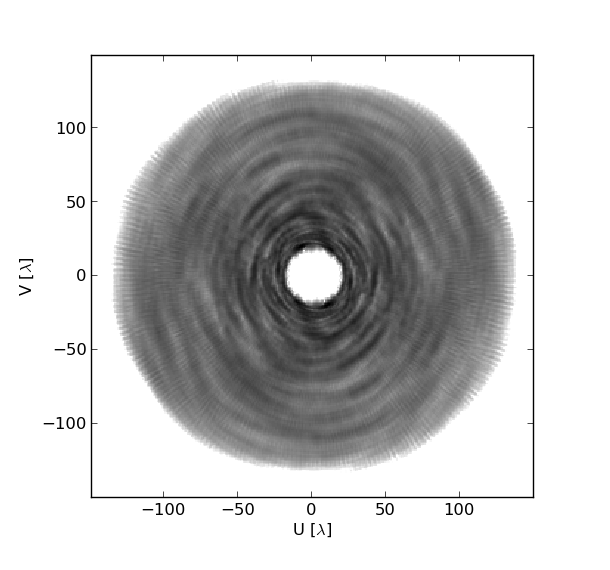
\includegraphics[width=0.9\textwidth]{plots/PicA_Oct2011_uv_coverage.png}
\caption{The effective uv coverage of a 10MHz-wide spectrum bin, showing the relative contributions of each baseline when beam-forming on Pictor over a 9.6 hour synthesis in the October observing session. \label{fig:uv_coverage}}
Not shown here are the weights interpolated from the Perley et al 330MHz map (Fig. \ref{fig:pic_perley}) used to recover the total integrated flux of Pic  which represent a few \% change on the longest baselines.
\end{figure}

The beam-forming method assumes the target is a point source. Our primary
target, Pictor A, is slightly resolved by PAPER, and merits closer attention.
Pictor A is a double-lobed radio galaxy with a main lobe separation of
7\arcmin. As we see in Figure \ref{fig:pic_perley}, it is nearly unresolved by
PAPER's 15\arcmin synthesized beam. However, given the high SNR of the
observations, we see a 20\% drop in flux on the longest ($\sim$300m) baselines. 
We account for this by weighting baselines
in the beamform step according to a model of structure observed by
\citet{Perley:1997p9312} at 330MHz, which they found to be consistent with
their more limited 74MHz images as well as the detailed high frequency maps.
The normalized image is Fourier transformed and sampled at the desired uv
spacing by spline interpolation. These samples are used to weight each baseline
contribution in the baseline sum. The result is an estimate of the total
integrated flux for Pictor A. Where the resolution is highest, at the top of
the band, the correction is 3\%. At the bottom of the band, where the
resolution size has grown to 19\arcmin, the correction is only 0.6\%. The
resulting spectrum is shown in Figure \ref{fig:pic_spectrum}a.



\begin{figure}
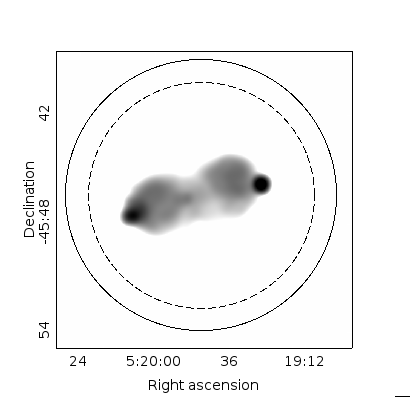
\includegraphics[width=0.96\textwidth]{plots/picA_Perley.png}
\caption{
Pictor A imaged at 330MHz by the VLA \citep{Perley:1997p9312}. Black circle
indicates PAPER resolution at the 150MHz, dashed, the resolution at 185MHz.  To
correct for the small residual structure in the PAPER measurements we resampled
the Perley image to the PAPER resolution and estimated the relative contribution
 to each PAPER baseline.  At the highest frequency this
led to a 3\% correction, at the lowest frequency, 0.6\%.
\label{fig:pic_perley}}
\end{figure}

%BANDPASS CALIBRATION
\subsection{Bandpass Calibration}
\label{sec:Calibration}

The resulting set of spectra were then calibrated to a model of J2331-416 to remove 
the residual bandpass due to the net effect of the primary beam as discussed in \S \ref{sec:approach}. J2331-416 
\footnote{Here we set the spectrum to $S_{150}=33$Jy, $\alpha=-0.76$} fit to measurements beolow 1GHz \citep{slee1995,kuhr_et_al1981,large_et_al1981,burgess_hunstead2006}.
was selected for its relatively high brightness, spectral smoothness and large quantity
 of available catalog data. Each source track has a slightly different sample profile
 resulting from different amounts of flagged data at each time and channel. To account
 for these differences in the bandpass calibration we build a set of calibration tracks 
 that match the tracks for each source. Calibration of each source then proceeds with
 an optimally matched calibration spectrum.



%The gain of each channel is the product of an overall instrumental passband and
%the spectral dependence of the primary beam in the direction of the source.
%Sources sharing the same track through the primary beam will have the same
%average spectral gain function resulting from frequency dependent primary beam
%attenuation.   We matched each measured source spectrum time sample to the
%nearest sample (in altitude/azimuth) of a calibrator source
%(J2331-416)\footnote{This source was chosen for the amount of data found in the
%literature and the apparent smoothness of the spectrum.}.  We then, average the
%% XXX clarify why one source used here, and more sources later 
%two matched data streams in time.  Since both tracks make the same slice
%through the primary beam, they will have the same average effective gain.
%Assuming a power law model for J2331-416 (33Jy $\alpha=-0.76$), we compute a
%% XXX I got these parameters for 2331: $S_{150}=31.9\ {\rm Jy}$, $\alpha=-0.69$ 
%% XXX forward reference section on fitting spectra for how this was derived for 2331
%bandpass gain.  After calibrating the raw 203 channel spectra with this
%bandpass, we average into 10MHz sub-bands between 120 and 180 MHz, computing
%the standard deviation as an estimate of the error. 

% XXX merge this with above
%To further improve these estimates, we derive an additional frequency-dependent gain parameter,
%smoothed on 10-MHz scales,
%that brings the spectrum of J2331-416 into closest agreement with a power-law spectrum of
%$S_{150}=31.9\ {\rm Jy}$, $\alpha=-0.69$ that represents the best fit to measurements below 1 GHz
%\citep{slee1995,kuhr_et_al1981,large_et_al1981,burgess_hunstead2006}.
%This additional gain factor was applied to all measured spectra, including that
%of Pictor A.  The expectation is that, since all sources at similar declinations follow similar tracks 
%through the PAPER beam, any errors present in the original measured spectra as a result of differences between
%the simulated and actual beam response should be absent in the ratio between source spectra, and therefore
%should be corrected by the applied gain factor


\subsection{Fitting a Power-Law Model to Spectra}


There is a variety of prior data at multiple wavelengths to which we want to calibrate
and then compare our measurements.  Our method for doing both of these steps
is to assume a basic spectral model relating the different catalog data points and
fit for spectral model and gain parameters. 

We estimate spectral model parameters and flux calibration in a
Bayesian way by calculating and marginalizing the posterior probability of the
catalog and new PAPER data.   This method
offers improved repeatability by specifying a single objective function that
represents the quality of the model fit and naturally defines the errors on the
parameters \citep{Hogg:2010p8759}.   See  \citet{Mackay:2003p9717}  or
\citet{Sivia:2006p9736} for more on Bayesian analysis methods and an excellent
astrophysical example by \cite{Press:1997p9783}. In brief, measurement errors
are related to parameter model errors via the likelihood, which we can calculate, 
and the posterior, which we cannot.  However, the posterior is theoretically
well sampled by a Markov Chain Monte Carlo sampler, which selects parameter
values at random, computes the likelihood of the model given the data and noise model,
and accepts or rejects the step based on an outside decision factor unrelated to the data.


Here we use the emcee sampler by \citet{Mackay:2003p9717} et al to generate chains of
parameter values. The best fit model is the median of all the sampled
parameter sets, while the volume containing a well defined fraction of samples
sets the confidence limits.  The oft quoted ``1$\sigma$" probability level
corresponding to a gaussian distribution contains 65\% of the samples. In
practice the contours are not gaussian. Here we choose a slightly more
conservative probability level of 76\% 


To model the relationship between different wavelengths we assume a single spectral index
which is the prevailing spectral energy distribution at low frequencies, 
though curvature or other
deviation from a power-law is not-uncommon.  

When fitting models to the full catalog, we use the Vollmer et al
catalog which has been optimally cross-matched at the expense of excluding more data points.
Meanwhile, the gain fit used a small sample of
sources with spectra which meet our calibration criteria: more precision data available,
brighter than most sources in the sample and far from any possibly confusing areas of
the sky. 
By limiting ourselves to a small number of sources we are able to go include catalog points by hand,
to avoid making the error of falsely including erroneously matched 
data points but benefiting from some measurements not included. 


\subsection{Approximating an Absolute Flux Scale}
\label{sec:flux_scale}

At the output of the beam forming and bandpass calibration step, the flux scale
 is tied to a model fit tp the catalog values of
J2331-416. The accuracy of this fit, and the implied uncertainty in the flux
scale, limits the accuracy of the PAPER measurements..  To refine the flux
scale and estimate our flux scale uncertainty, we bootstrap a single global flux scale 
correction factor using 5
sources selected for their brightness, spectral linearity and data
availability\footnote{Calibration sources:
2250-412,2331-416,2140-434,0007-446,0704-427}. To build a more complete
spectral model we go beyond the data found in Vollmer et al, including all spectral
measurements below 2GHz found in the NED database \footnote{\url{ned.ipac.caltech.edu}: Accessed 1 April 2013}.  These catalog measurements
are primarily by Parkes, and Molonglo with the best precision coming from the
Wills fluxes at 538 and 634 MHz (when available). Where error bars are not
given, we assume uncertainty of 25\%. 

Using the MCMC method we fit spectral index models to the catalog fluxes
 simultaneously with a global PAPER flux scale factor using  an MCMC chain to calculate the log likelihood

\begin{align}
\log\mathcal{L}_s &= \sum_{\nu}\frac{ (S_\textrm{cat}^{\nu}  - S_{150}  \left(\frac{\nu}{150}\right)^\alpha)^2}{2(\Delta S_\textrm{cat}^\nu)^2} +
\frac{ (g*S_\PAPER^{\nu}  - S_{150}\left(\frac{\nu}{150}\right)^\alpha)^2}{2(\Delta S_\PAPER^\nu)^2}\\
\log\mathcal{L} &= \sum_{s} \log\mathcal{L}_s
\end{align}


which samples the posterior probability of PAPER data ($SPAPER_{\nu}$) and
catalog values ($Scat_{\nu}$) given a spectral index model for each source and
a global flux scale factor ($g$) ($S_\PAPER^\textrm{calibrated} = g S_\PAPER$).
Marginalizing over the fitted flux scales, we find the resulting flux scale distribution function which is shown in Figure
\ref{fig:gain}. The 76\% confidence limit on this flux scale, relative to the
J2331-413 calibration, is  $-0.01 ^{+0.11}_{-0.17}$ dB, or a 3.24\%
multiplicative error on every calibrated PAPER measurement.  These errors are added, in quadrature,
to the errors in the PAPER spectra.


These calibrated spectra are plotted in Figures \ref{fig:srcs1},\ref{fig:srcs2},
\& \ref{fig:srcs3} and the data are listed in Table \ref{tab:data}.  The
resulting Pictor A spectrum ranges in precision from 6.5\% at 125MHz to 4.7\%
at 185MHz. At least half of this error is due to uncertainty in the flux scale.  

%The Pictor track is calibrated to 2331-416 ($S_{150}=33.8$Jy,$\alpha=-0.76$) and the Hydra A track to 0231-126 ($S_{150}=21$Jy,$\alpha=-0.7$).  
%    cal['0213-132'] = 21 * (fq/.150)**-0.7  
%    cal['1932-464'] = 93.7 * (fq/.150)**-0.82 
%    #cal['2331-416'] = 31.9 * (fq/.150)**-0.69
%    cal['2331-416'] = 33.9 * (fq/.150)**-0.76
%COMPARISON WITH DATA


\subsection{Fitting Spectral Models}
\label{sec:fitting_models}

Finally we compare all of our  calibrated spectra to catalog measurements. Our method
will be to first establish a best fit model to existing data, then add the PAPER data
to the fit, and assess the degree to which the PAPER data is supported by prior measurements, or the reverse
the degree to which PAPER offers an improvement in our knowledge of the spectrum.

 To establish the baseline model, we
fit a spectral model to catalog data from the spectrally and spatially
cross-matched meta-catalog by \citet{Vollmer:2010p6422} using the
 (log) likelihood which assumes Gaussian measurement errors

\begin{equation}
\logL = \sum_\nu{\frac{\left(S_\nu - S_{150}\left(\frac{\nu}{150}\right)^\alpha\right)^2}{\Delta S_\nu} }
%\label{eq:catlogL}
\end{equation}


We estimate the confidence interval of the resulting parameters as the boundary
enclosing 76\% of the samples. In the catalog we report both the upper and
lower of these values for both parameters and plot the 2D contour to show the
correlation of the two parameters. Many of these contours, the grey curves in
Fig. \ref{fig:SI_contour_1}, are classic banana plots, displaying a non-linear
correlation between the parameters.    In most cases the single contour
adequately describes 2D posterior distribution.

Confidence contours for
the complete set are shown in grey in Figs. \ref{fig:SI_contour_1} -
\ref{fig:SI_contour_4}.  In general these are lower limits on the possible
precision, as the Vollmer catalog emphasizes minimization of cross-match error
but at the cost of excluding data points.  The fit is then performed again with
both PAPER and catalog data, shown in black on the same Figures. The values are
given in Table \ref{tab:fits}, and
illustrated in Figure \ref{fig:src_spec}.  






\begin{figure}[htbp]
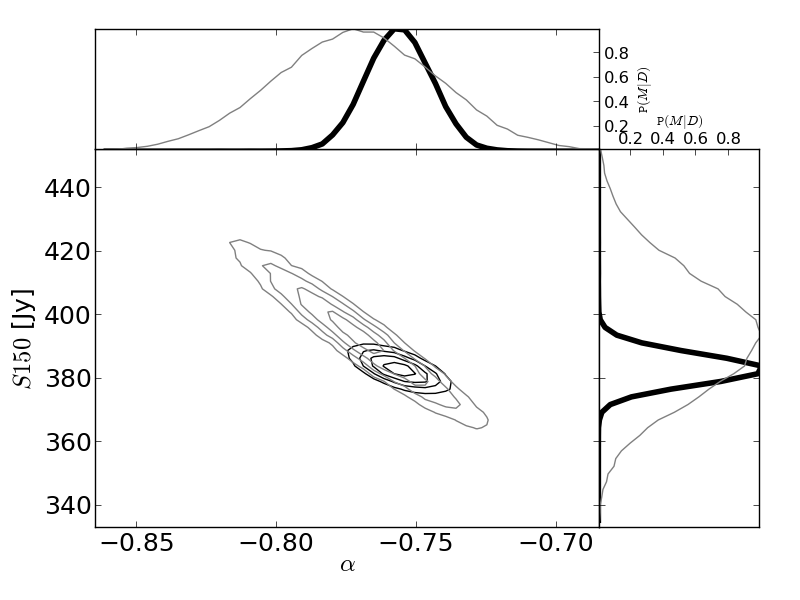
\includegraphics[width=0.49\textwidth]{plots/pic_trace_hist.png}
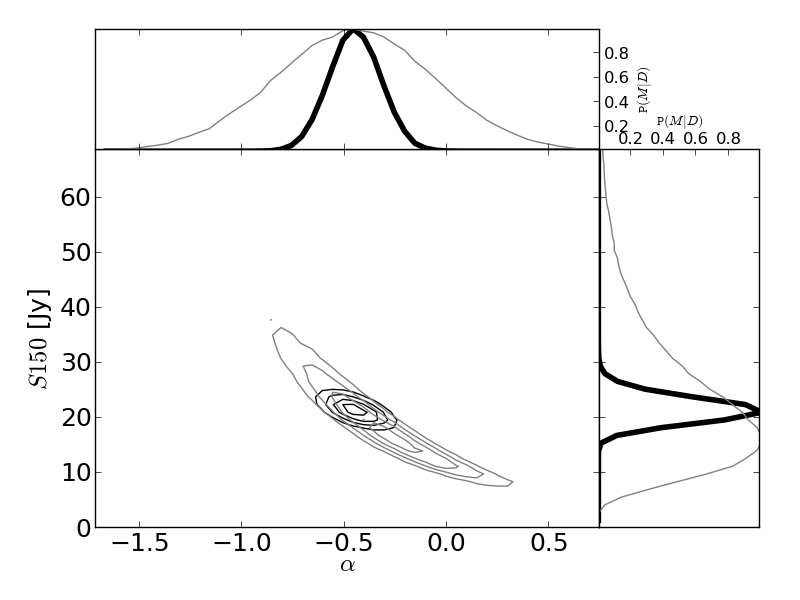
\includegraphics[width=0.49\textwidth]{plots/1556-466_trace_hist.png}
\caption{
A more detailed view of the posterior probability distribution. On the left
Pictor A, on the right 1556-466. Confidence contours range from 0.2 to 0.8.
Compare with the contours for this source shown in Fig. \ref{fig:SI_contour_3}.
As above, grey for  the fit to catalog data, black for joint catalog and PAPER
fit.
}
\end{figure}




\section{Results and Discussion}
\label{sec:fits}

%0008-421#
%1243-412#
%1247-401#
%1315-460
%TODO round up the source counts

In the 59 sources measured, four demonstrated poor convergence fitting a single
spectral index to both the PAPER data and prior catalog data. In three
cases\footnote{1243-412,1247-401,1315-460} %TODO update these sources are in
the Centaurus A/galactic plane region. Though the beam forming method provides
relatively high dynamic range of $\sim$100:1 it is unable to distinguish
between these sources and the bright diffuse Centaurus and galactic structure.
The last source, 0008-421, was not detected by previous PAPER observations and
exhibits flattening at higher frequencies, most likely due to synchrotron
self-absorption \citep{Jacobs:2011p8438} .  The remaining 94\% MCMC chains
arrived at a stable posterior distribution. The spectral index parameters for
these chains are given in table \ref{tab:fits}.

Inspecting the confidence contours we find that, for the vast majority ($\sim
75$\%), the PAPER measurements confirm the power law extrapolation from higher
frequencies. The remaining 25\% either A) have large PAPER error bars and
therefore provide no new information or B) do not agree with the spectral index
model.  To understand where most measurements fall on this spectrum we
numerically quantify the overall model improvement derived from the addition of
the PAPER data as 
\begin{align}
\textrm{Improvement} &= \left(\textrm{Precision increase}\right) \left(\textrm{Catalog agreement}\right)\\
&= \left(\frac{1}{Area(\textrm{PAPER})} - \frac{1}{Area(\textrm{Cat})}\right) \left( Area(\PAPER \cap \textrm{Cat}) \right)
\end{align}

We quantify the fit {\em precision increase} as the change in the contour
figure of merit, defined as the inverse area of the confidence contour.
Meanwhile, {\em catalog agreement} is the fraction of the PAPER confidence
interval that overlaps the catalog confidence interval.  Thus, for example, in
a PAPER fit that overlaps the catalog confidence contour by 41\% but increases
in precision (confidence area shrinks) by a factor of 3, the resulting {\em
improvement} will be 0.123.  

In these sources, the improvement index ranges from a max of 6.9 to -0.022.
10\% of sources showed negative improvement, suggesting that PAPER data have
added to uncertainty (see Figure \ref{fig:SI_contour_bad}). 12\% of sources
have exactly zero improvement, which indicates that the PAPER data have pulled
the fit far from the model preferred by the catalog data (see Fig.
\ref{fig:SI_contour_new}).  The spectral models of these sources have not been
included in Table \ref{tab:fits}.  The remainder of the spectral fits are
included for completeness, but given the range of quality found, particularly
near the Galactic plane and Centaurus A, should be used with utmost caution.

However, the majority of source 78\% have positive improvement index,
indicating strong confirmation of the extrapolated spectrum (see Figures
\ref{fig:SI_contour_1} - \ref{fig:SI_contour_4}).  Pictor A is in the middle of
this group  with an improvement of 0.39 ---only 14 sources show stronger
confirmation.  The flux model is $S150=$388 $\pm$ 9.4Jy, $\alpha=-0.77\pm0.02$.
The combination of several independent PAPER data points near 150MHz with
previous catalog measurements results in this estimated uncertainty of 2.4\%.
This uncertainty is dominated by agreement between the 2 Wills measurements
near 600MHz which are accurate to 2\% and the five PAPER measurements, which
are accurate to ~5\%.  This error estimate includes an estimate of accuracy of the overall flux scale,
as well as the source-source variation due to primary beam errors. 


% XXX comparison with previous in-band results (danny 2011, williams 2012)
% work TODO

 \section{Conclusion}
 \label{sec:Conclusion}

Here we have provided a measurement of Pictor A with enough precision to confirm
a highly linear spectral index between 150 and 600MHz. We then used the same
filtered beam form method to measure the spectra of bright sources with similar
primary beam response. This primary beam limit is based on our measurements 
of the primary beam along slices of constant declination.  


The measurements provided
here are the first, calibrated, broad-band spectra to cover the EoR band. Existing EoR band measurements
are accurate to 20\% implying a 40\% uncertainty in the absolute power spectrum
level.  The Pictor A spectrum here is shown to be accurate to 
$\sim$5\%, a factor of 5 improvement over previous measurements.

This uncertainty includes the 
variation in each PAPER measurement ($\sim$1\%), variation between sources and the errors resulting
from extrapolating the \citet{Baars:1977p9678} scale beyond its original range. These last
two are found simultaneously by fitting the spectral extrapolations of several flux calibrators
at once and account for the the majority of the error. Though past measurements suggested the possibility
of spectral curvature below 200MHz we have found no evidence for this.  With these measurements we are able 
to confirm single spectral index model for Pictor between 120MHz and 600MHz.

A set of  61 verification sources were selected to be bright, previously cataloged
and  distributed over
the full 24 hours of Right Ascension coverage but only within 5 degrees
declination of Pictor A.  Using a Bayesian analysis we conclude that most of
these are consistent with previous measurements and provide useful new
constraints. However, in a small remainder, the simple spectral model fails to
adequately describe the data. In most cases the proximity to bright or extended
structures implies side lobe contamination.  Therefore, though we include the
model parameters, they are not meant to be definitive, but provide confidence
that the reported PAPER flux values are on the correct global scale.


Direct measurements of the Pictor A spectrum are key to correctly setting the
flux scale of PAPER, MWA and future EoR experiments like the Hydrogen Epoch of Reionization Array (HERA).
These spectra provide tighter constraints on many of the EoR band fluxes, while
limiting the pernicious affect of primary beam uncertainty.  Future work will use these
fluxes to further  refine the primary beam models of these experiments which is crucial to properly reconstructing
both image and power spectrum flux.


\begin{figure*}
\centering
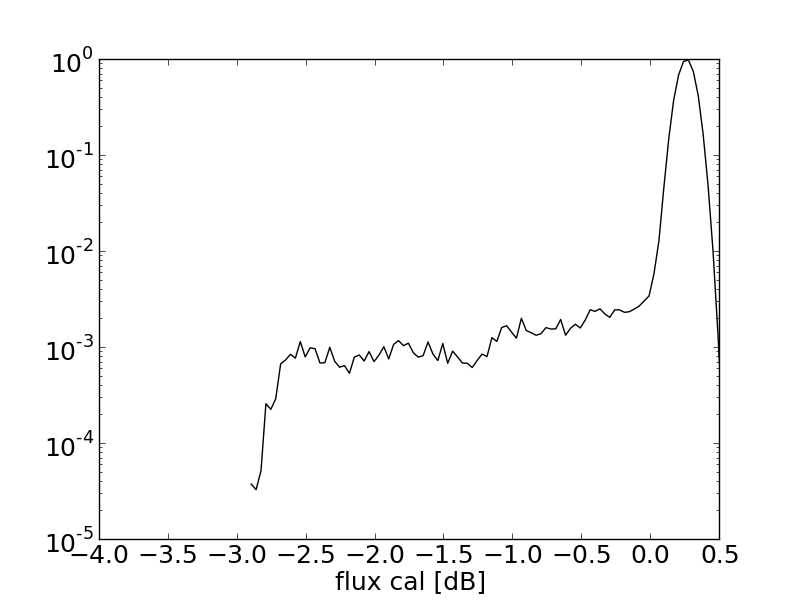
\includegraphics[width=0.9\textwidth]{plots/1526-423_2250-412_2331-416_1932-464_1421-490_gain_mcmc_chain_gain_conf.png}
\caption{
The marginalized PAPER flux scale factor posterior probability distribution
function bootstrapped from the NED database listings for
2250-412,2331-416,2140-434,0007-446 and 0704-427 below 2GHz.
\label{fig:gain}}
\end{figure*}

\begin{figure*}[htbp]
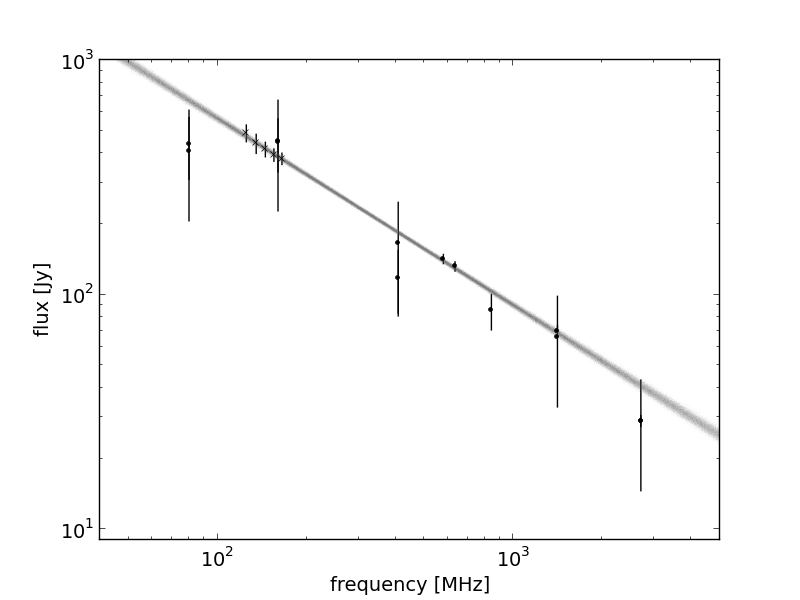
\includegraphics[width=0.49\textwidth]{plots/pictor_spectrum.png}
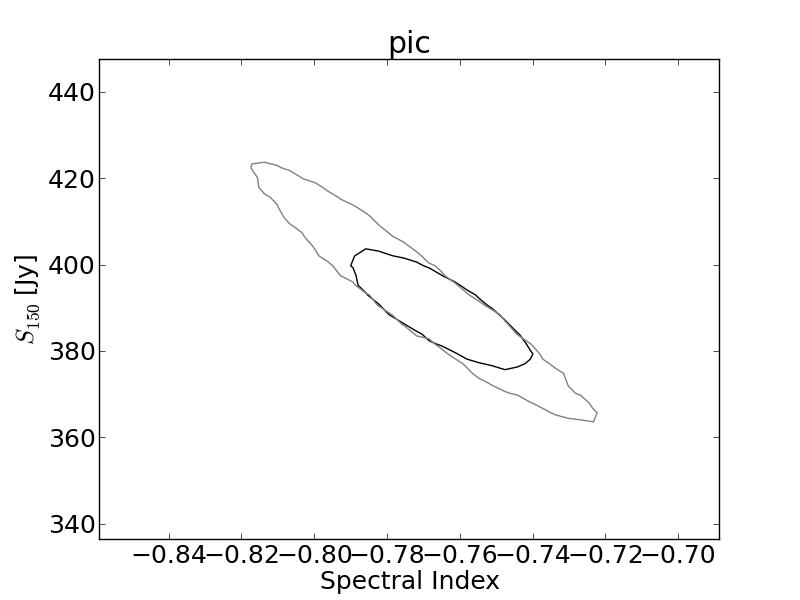
\includegraphics[width=0.49\textwidth]{plots/pic_SI_MCMC.png}
\caption{
Using new PAPER results to constrain the spectrum of Pictor A.  On the left,
the PAPER Pictor A spectrum with 2$\sigma$ error bars (x) and  MCMC fits (grey
cloud). Inset allows comparison between the 10MHz averaged points with the
403kHz points (grey). The oscillations in the PAPER spectrum are residual side
lobe contamination from other sources and are well represented by the error
bars.  The most reliable prior measurements (dots) are those by
\cite{Wills:1975p9314} at 580MHz and 635MHz \citep{Perley:1997p9312}. The rest
are from with Culgoora \cite{Slee:1995p7541} or Parkes
\cite{Otrupcek:1991p8780} and have been set to the (extrapolated)
\citet{Baars:1977p9678} scale by  \cite{Kuehr:1981p9628}. A sub-sample of MCMC
fits are shown in blue. On the right, the grey contour indicates the 76\%
confidence interval for 150MHz flux and spectral index given the prior data.
Black folds in the PAPER data.
} \label{fig:pic_spectrum}
\end{figure*}

%%calibrators
%%2250-412_2331-416_0043-424
%\begin{figure*}[htbp]
%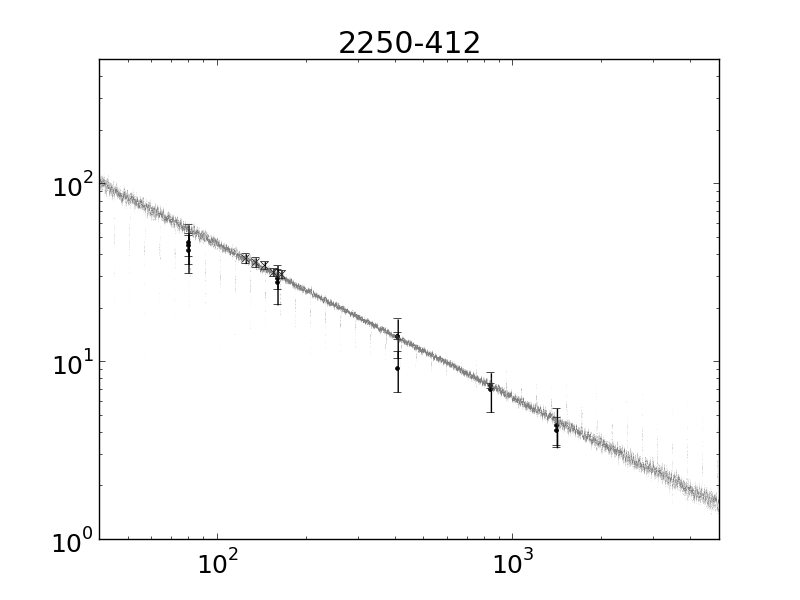
\includegraphics[width=0.2\textwidth]{plots/2250-412_calfit.png}
%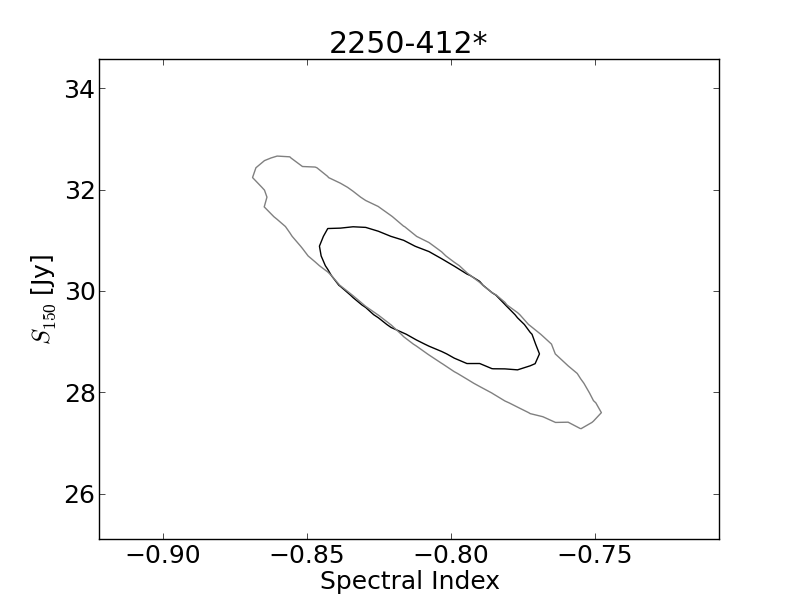
\includegraphics[width=0.2\textwidth]{plots/2250-412_SI_MCMC.png}
%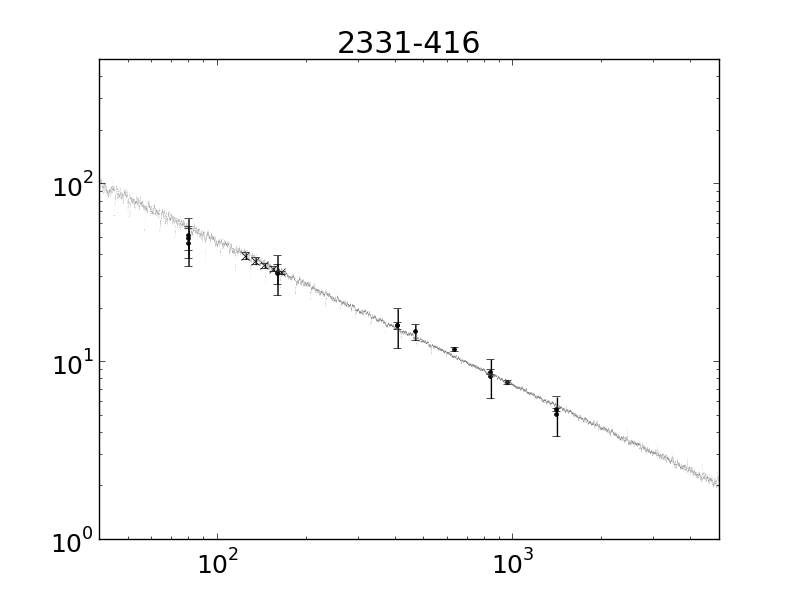
\includegraphics[width=0.2\textwidth]{plots/2331-416_calfit.png}
%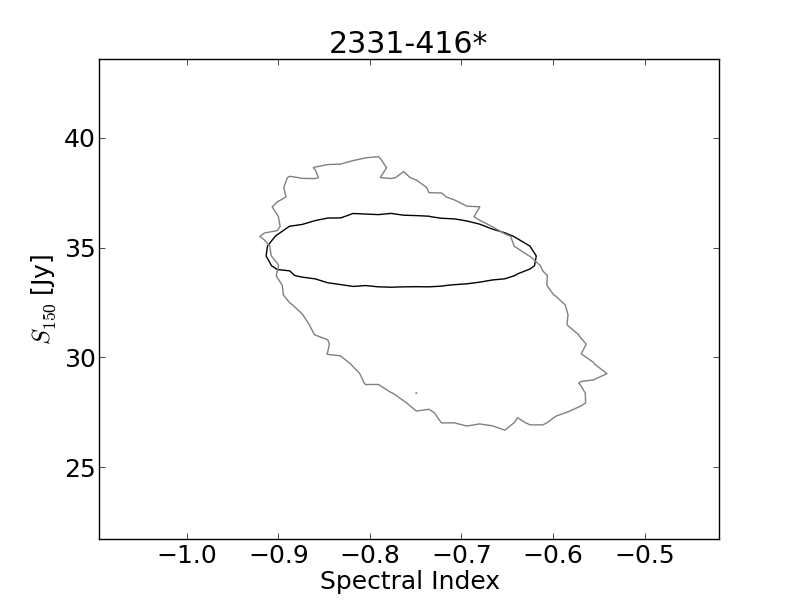
\includegraphics[width=0.2\textwidth]{plots/2331-416_SI_MCMC.png}\\
%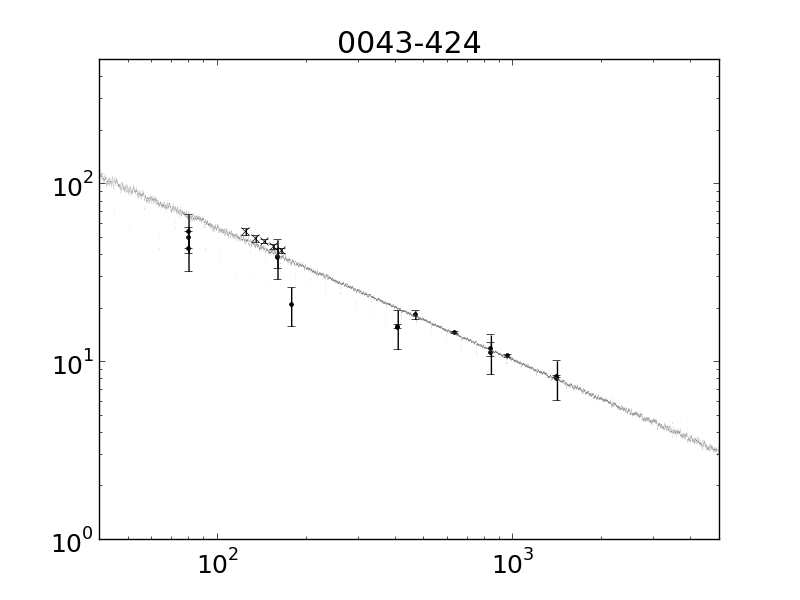
\includegraphics[width=0.2\textwidth]{plots/0043-424_calfit.png}
%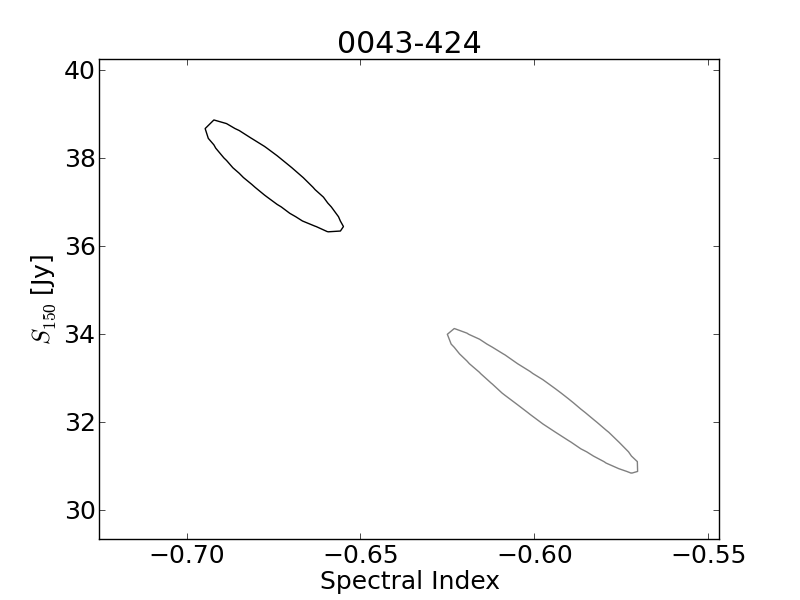
\includegraphics[width=0.2\textwidth]{plots/0043-424_SI_MCMC.png}
%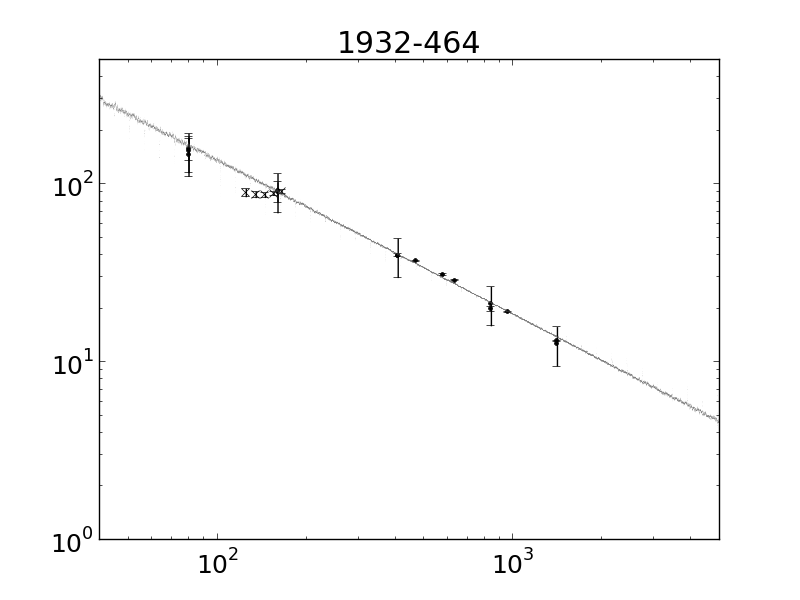
\includegraphics[width=0.2\textwidth]{plots/1932-464_calfit.png}
%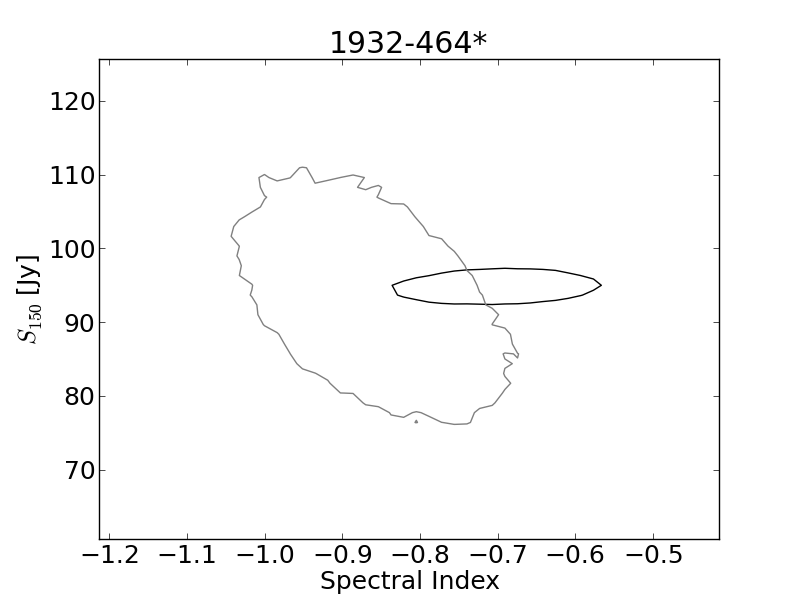
\includegraphics[width=0.2\textwidth]{plots/1932-464_SI_MCMC.png}
%
%\caption{Sources used to calculate the flux scale. Catalog data for the three sources are used to simultaneously fit a 
%single spectral index gain model for each source (grey contours) and a single PAPER gain parameter  .\label{fig:cals} }
%
%\end{figure*}
%add calibrator



\section*{Acknowledgements}

The PAPER project is supported by the National Science Foundation (awards
0804508, 1129258, and 1125558), and a generous grant from the Mt. Cuba
Astronomical Association.

This work makes use of ]the ``MCMC Hammer" emcee python library \citep[
\url{http://danfm.ca/emcee/}]{ForemanMackey:2012p8684}  and the NASA/IPAC
Extragalactic Database (NED) which is operated by the Jet Propulsion
Laboratory, California Institute of Technology, under contract with the
National Aeronautics and Space Administration.



\begin{figure*}[htbp]
\begin{center}
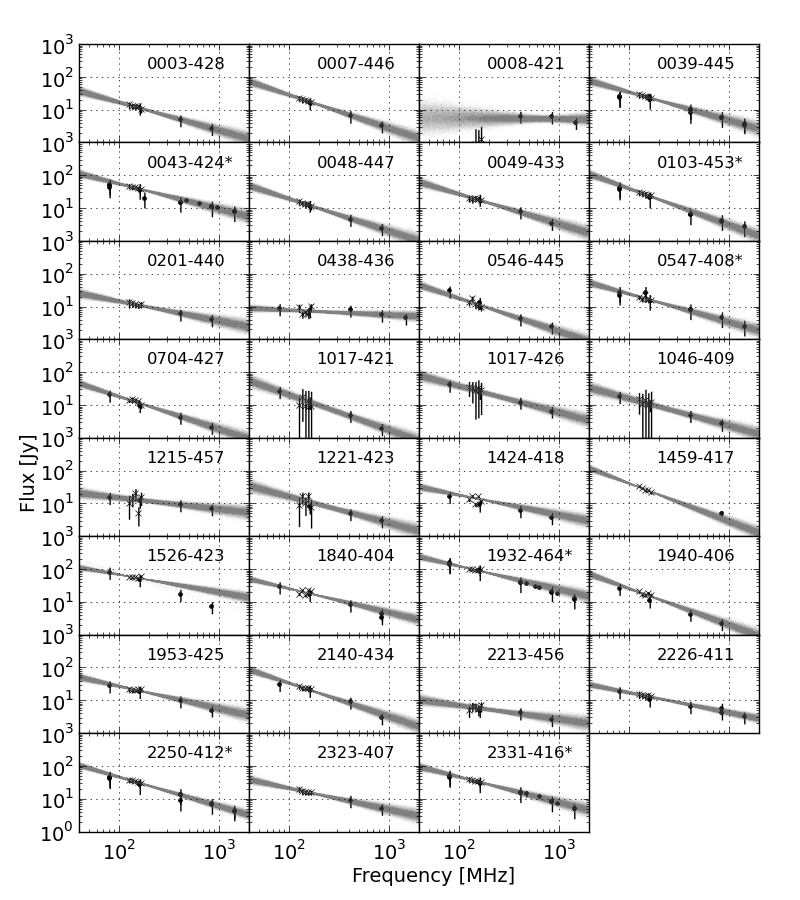
\includegraphics[width=0.9\textwidth]{plots/srcfig_1.png}
\end{center}
\caption{
PAPER spectra of 16 sources compared against existing data out of
\cite{Vollmer:2010p6422} between 40MHz and 2GHz, otherwise as described in
Figure \ref{fig:pic_spectrum}.\label{fig:srcs1}. Sources used to bootstrap the
flux calibration are noted with a *.
}
\end{figure*}

\begin{figure*}[htbp]
\begin{center}
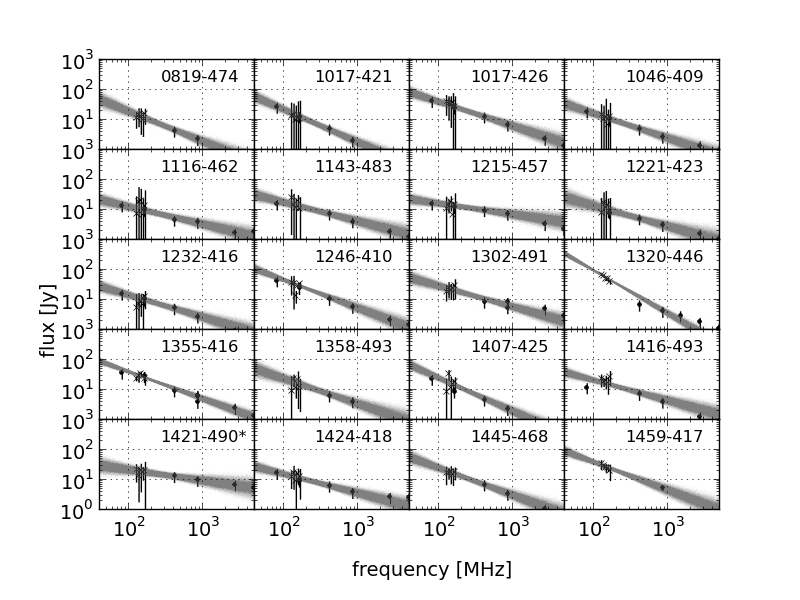
\includegraphics[width=0.9\textwidth]{plots/srcfig_2.png}
\caption{
PAPER spectra of 16 sources compared against existing data out of
\cite{Vollmer:2010p6422} between 40MHz and 2GHz, otherwise as described in
Figure \ref{fig:pic_spectrum}.\label{fig:srcs2} Sources used to bootstrap the
flux calibration are noted with a *.
}
\end{center}
\end{figure*}

\begin{figure*}[htbp]
\begin{center}
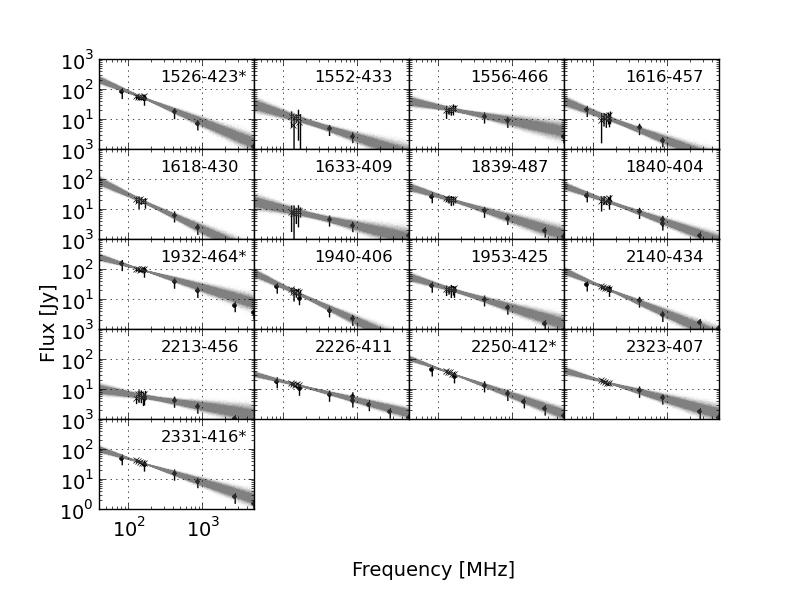
\includegraphics[width=0.9\textwidth]{plots/srcfig_3.png}
\caption{
PAPER spectra of 16 sources compared against existing data out of
\cite{Vollmer:2010p6422} between 40MHz and 2GHz, otherwise as described in
Figure \ref{fig:pic_spectrum}.\label{fig:srcs3} Sources used to bootstrap the
flux calibration are noted with a *.
}
\end{center}
\end{figure*}



%(PAPER_imaging)danny@keynes:plots$ python sort_SI_plots.py psa64_pic_stripe_perleycorr_SEDfits.txt
%TOP OF MAIN CONFIDENCE PLOT SECTION
%the best sources. High quality fit that improves on previous knowledge
\begin{figure*}[htbp]
\begin{center}
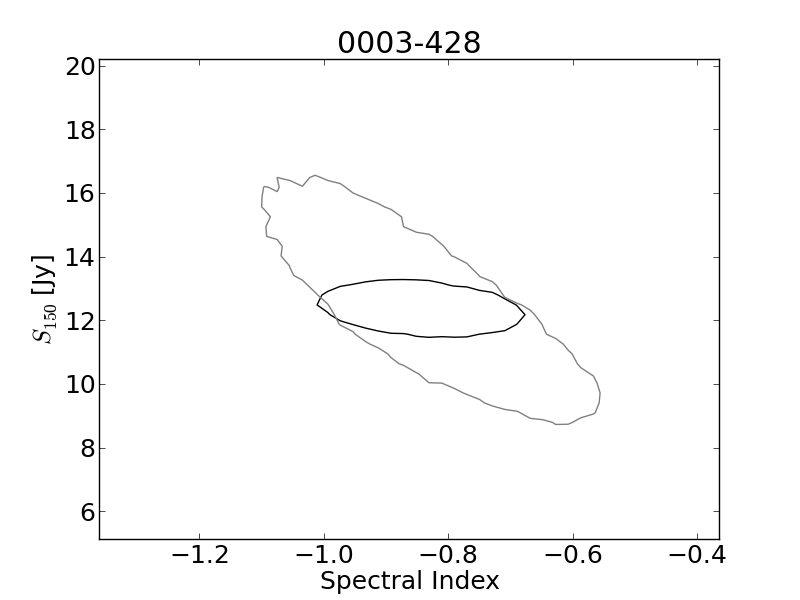
\includegraphics[width=2in]{plots/0003-428_SI_MCMC.png} %0.9878
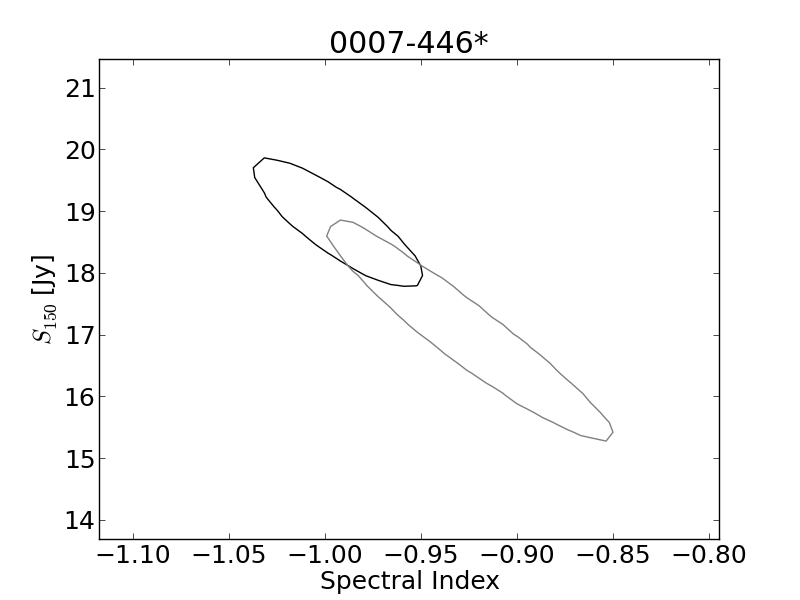
\includegraphics[width=2in]{plots/0007-446_SI_MCMC.png} %1.0085
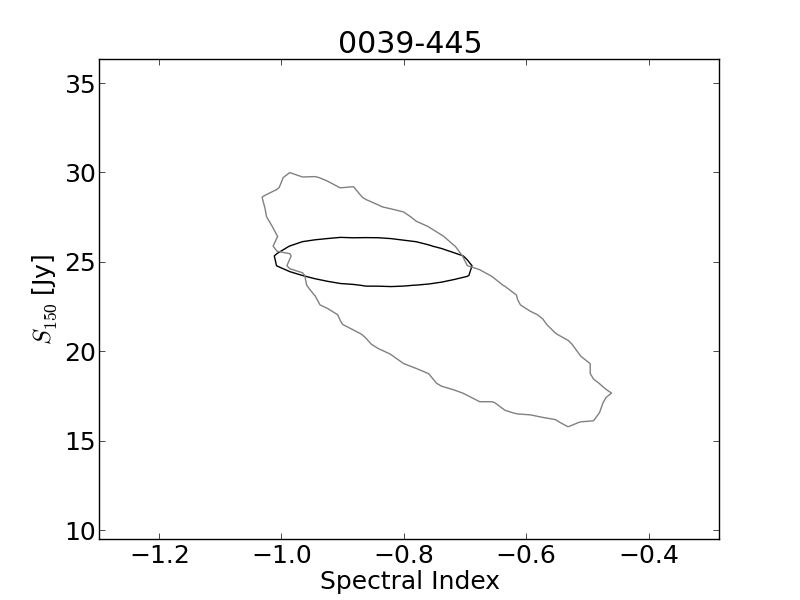
\includegraphics[width=2in]{plots/0039-445_SI_MCMC.png} %1.3403
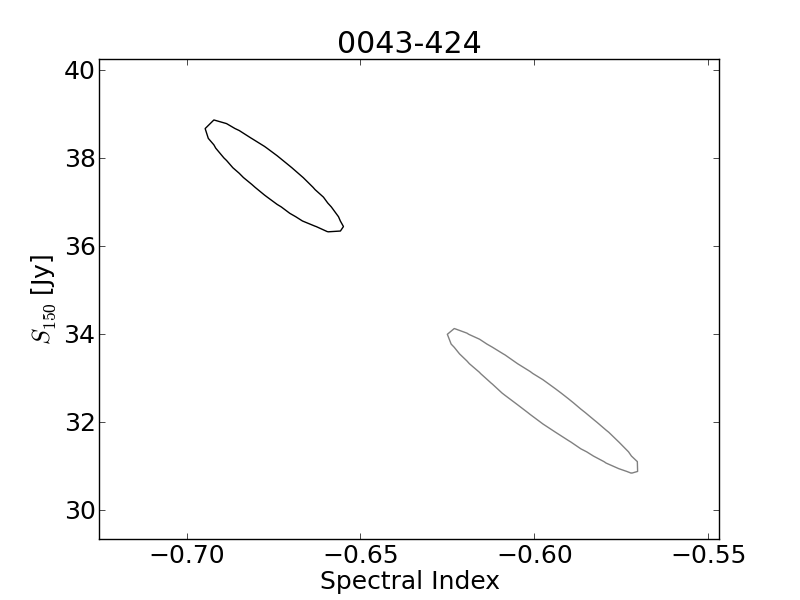
\includegraphics[width=2in]{plots/0043-424_SI_MCMC.png} %0.5959
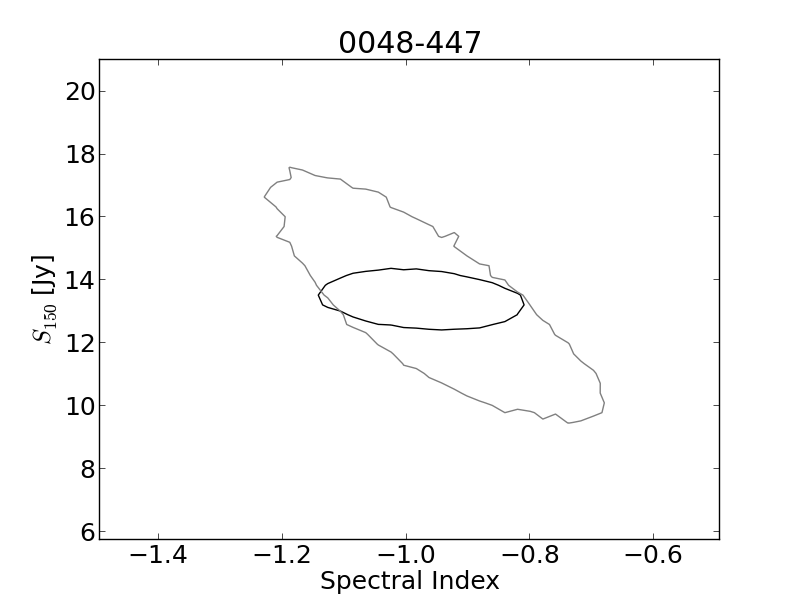
\includegraphics[width=2in]{plots/0048-447_SI_MCMC.png} %0.6165
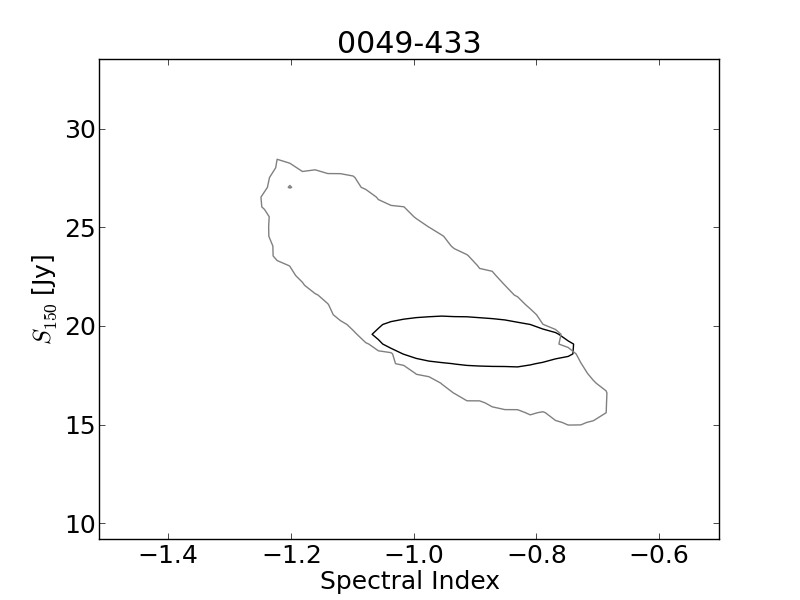
\includegraphics[width=2in]{plots/0049-433_SI_MCMC.png} %1.0632
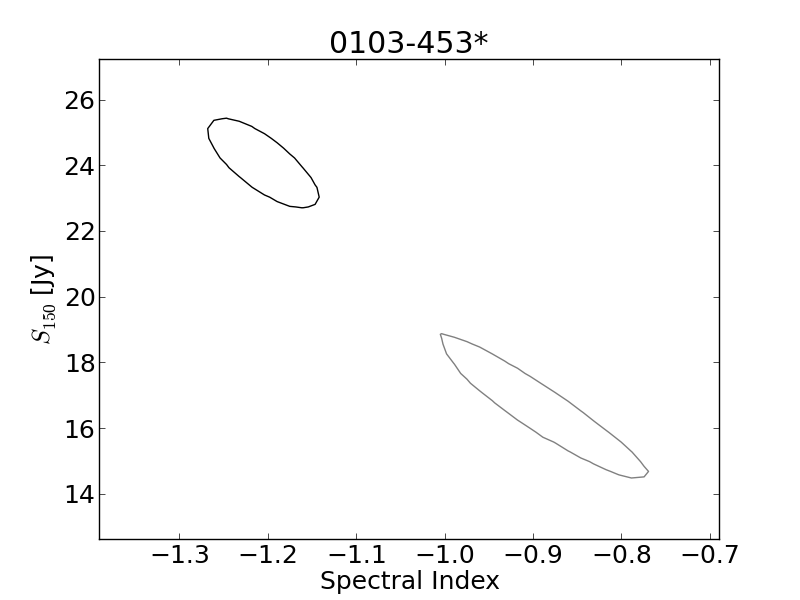
\includegraphics[width=2in]{plots/0103-453_SI_MCMC.png} %0.1456
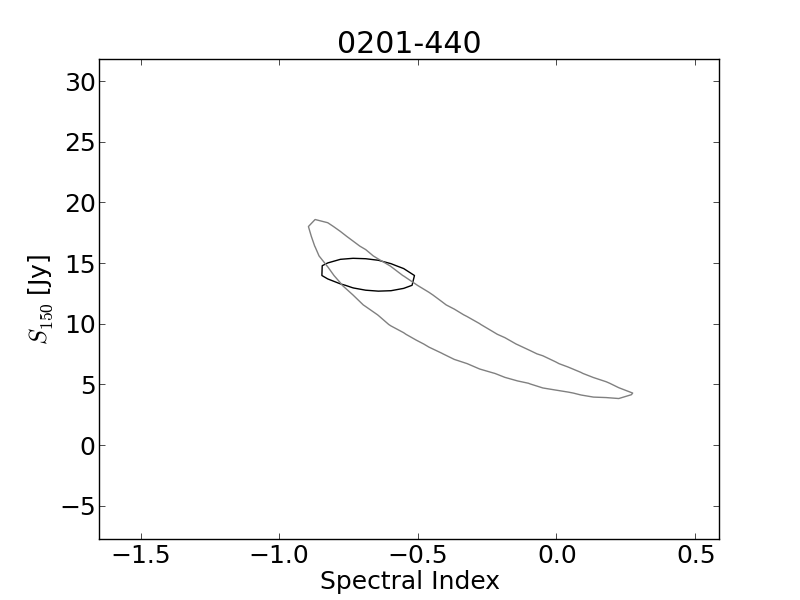
\includegraphics[width=2in]{plots/0201-440_SI_MCMC.png} %3.0727
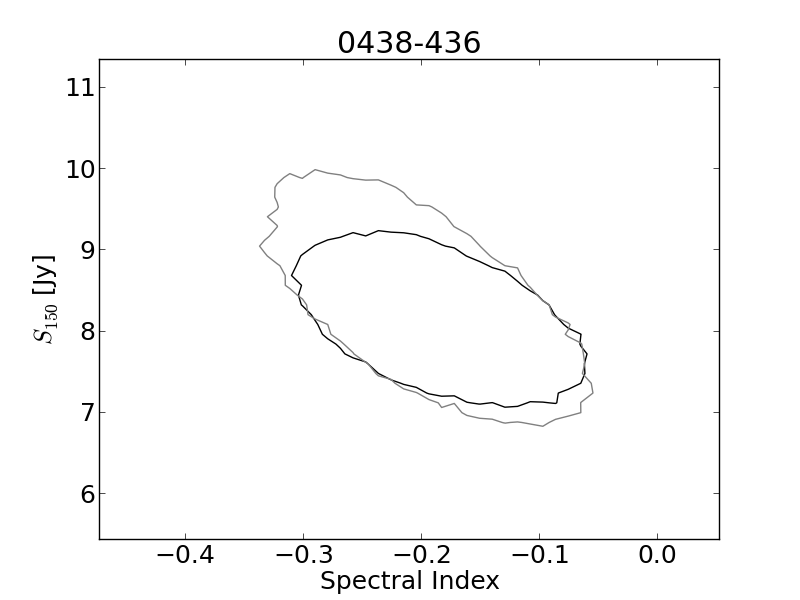
\includegraphics[width=2in]{plots/0438-436_SI_MCMC.png} %0.0991
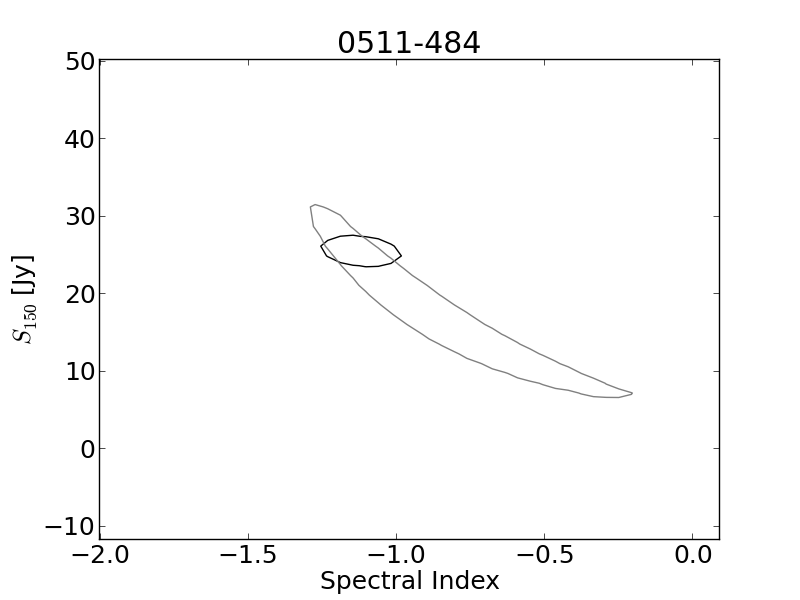
\includegraphics[width=2in]{plots/0511-484_SI_MCMC.png} %3.3967
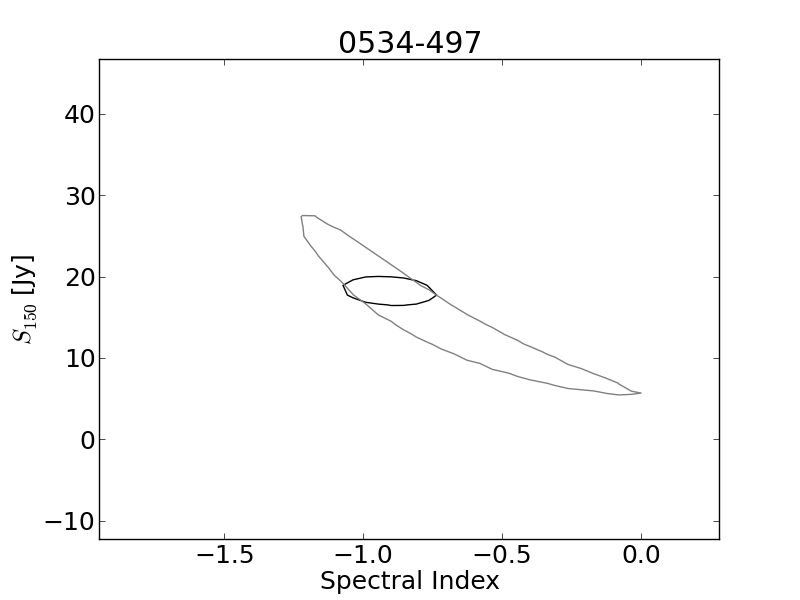
\includegraphics[width=2in]{plots/0534-497_SI_MCMC.png} %3.4118
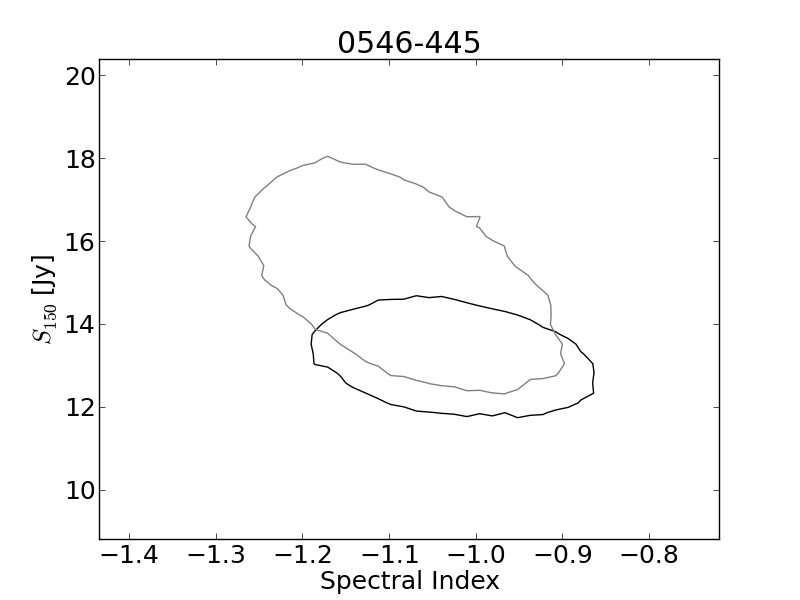
\includegraphics[width=2in]{plots/0546-445_SI_MCMC.png} %0.1647
\end{center}
\caption{Spectral model contours as described in Figure \ref{fig:pic_spectrum}. Sources marked with a
* were used to assess calibration error.
}\label{fig:SI_contour_1}
\end{figure*}
\clearpage
\begin{figure*}[htbp]2\begin{center}
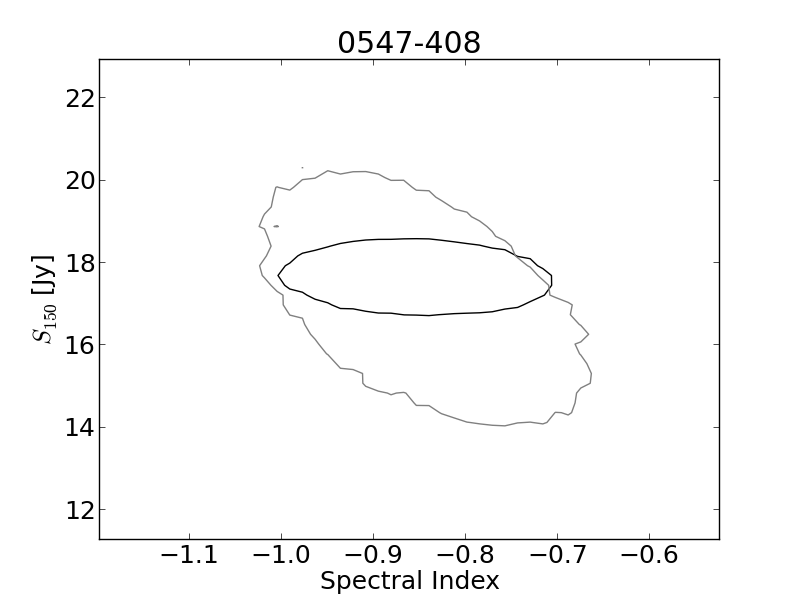
\includegraphics[width=2in]{plots/0547-408_SI_MCMC.png} %0.1506
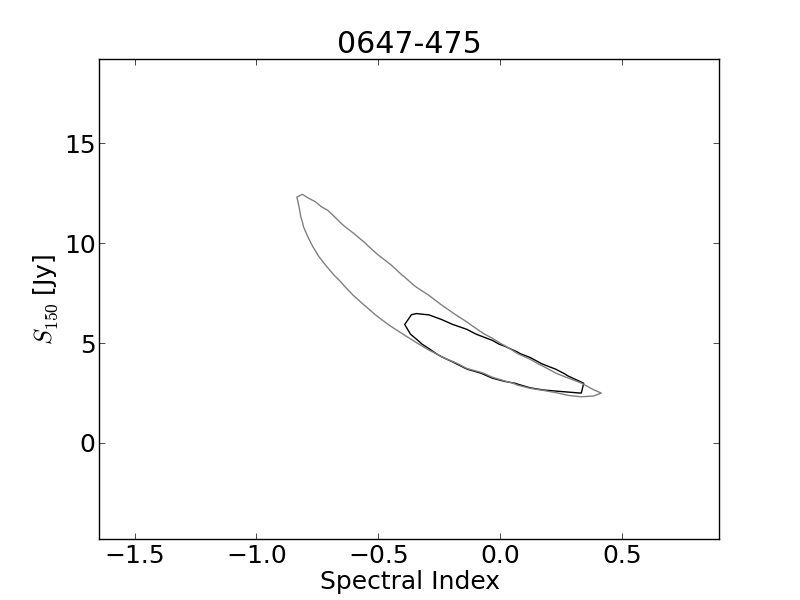
\includegraphics[width=2in]{plots/0647-475_SI_MCMC.png} %0.8384
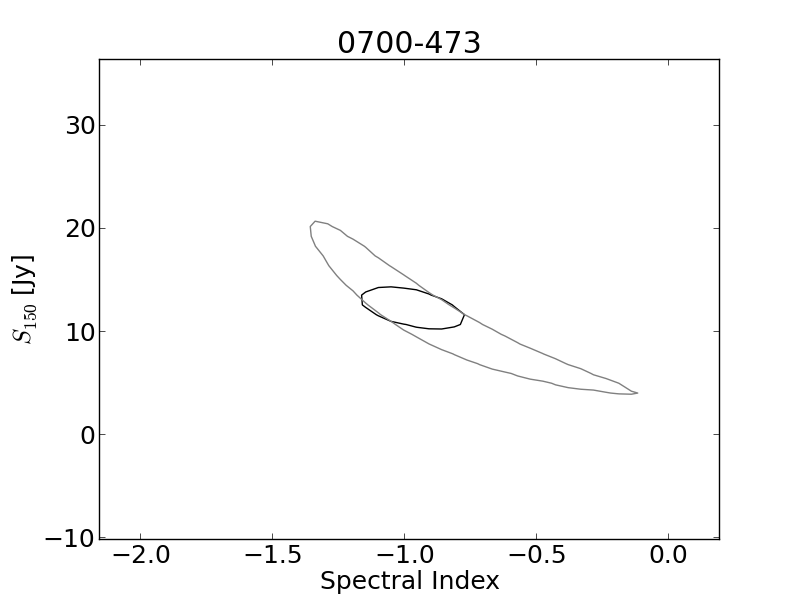
\includegraphics[width=2in]{plots/0700-473_SI_MCMC.png} %1.9848
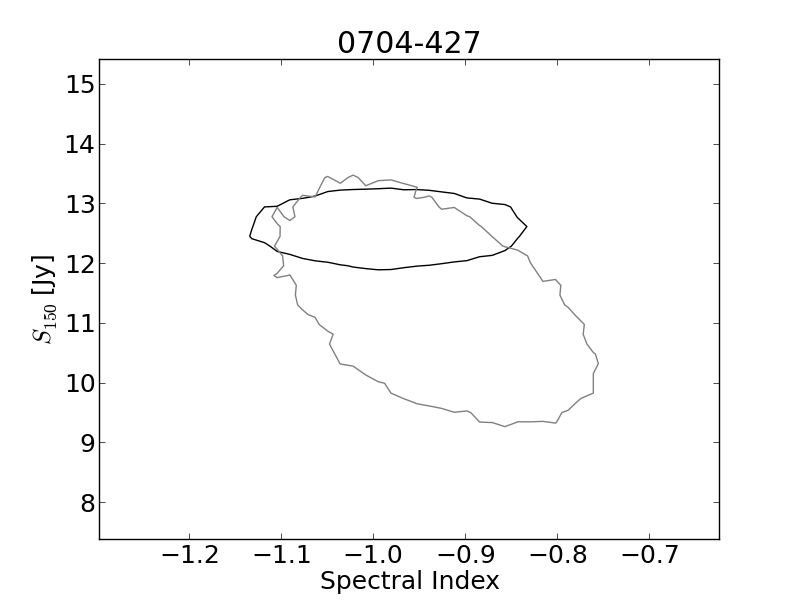
\includegraphics[width=2in]{plots/0704-427_SI_MCMC.png} %0.0785
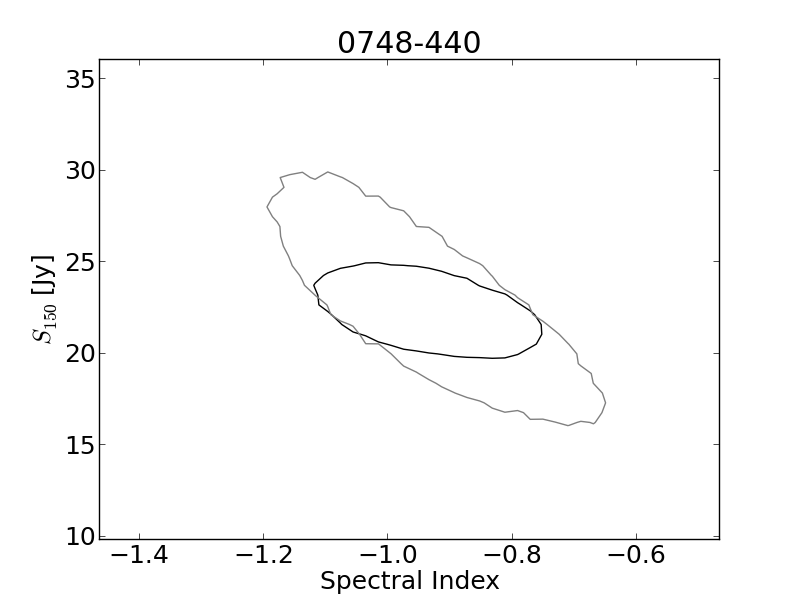
\includegraphics[width=2in]{plots/0748-440_SI_MCMC.png} %0.2942
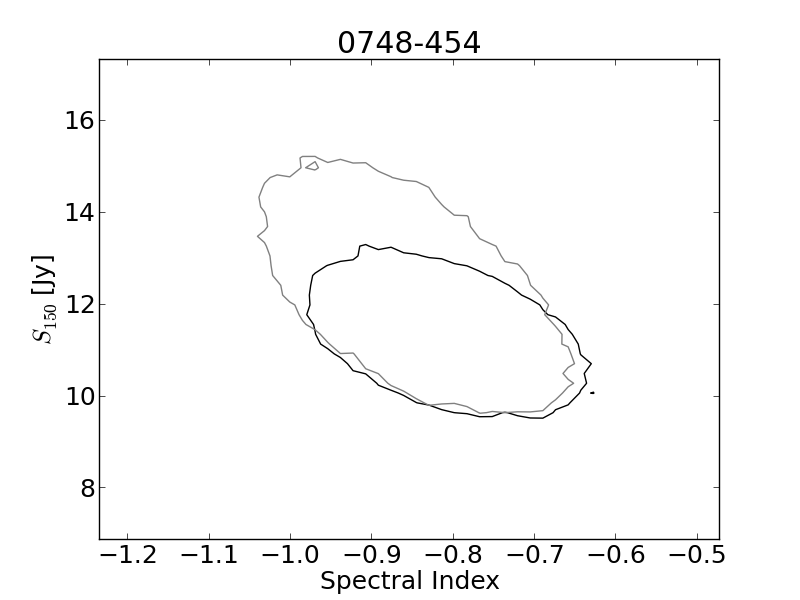
\includegraphics[width=2in]{plots/0748-454_SI_MCMC.png} %0.0742
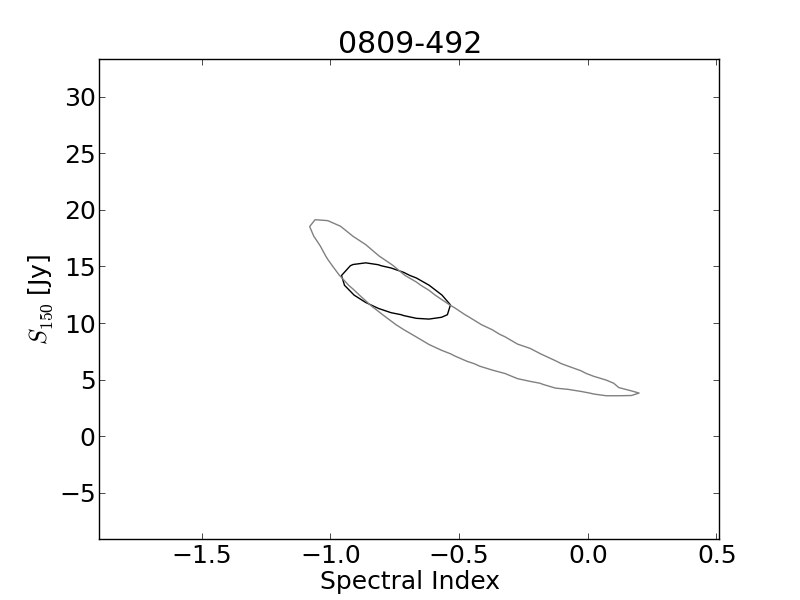
\includegraphics[width=2in]{plots/0809-492_SI_MCMC.png} %0.6265
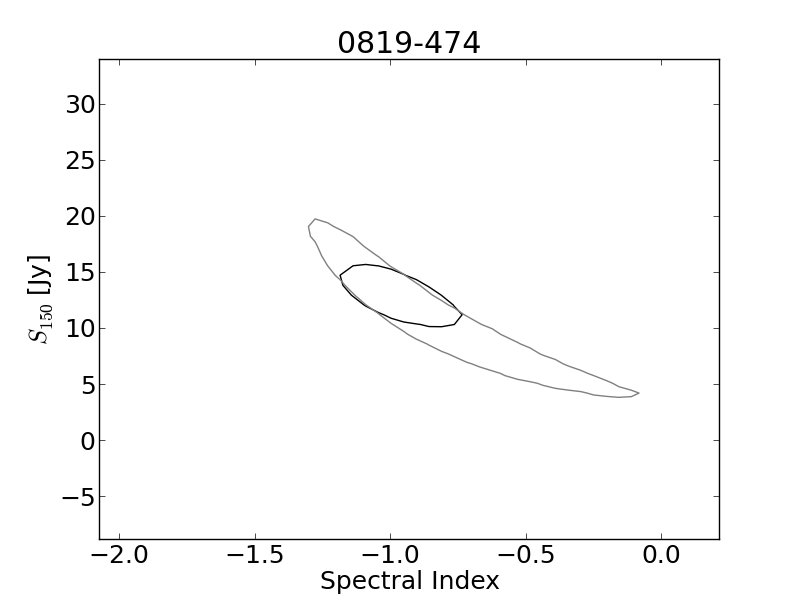
\includegraphics[width=2in]{plots/0819-474_SI_MCMC.png} %0.9749
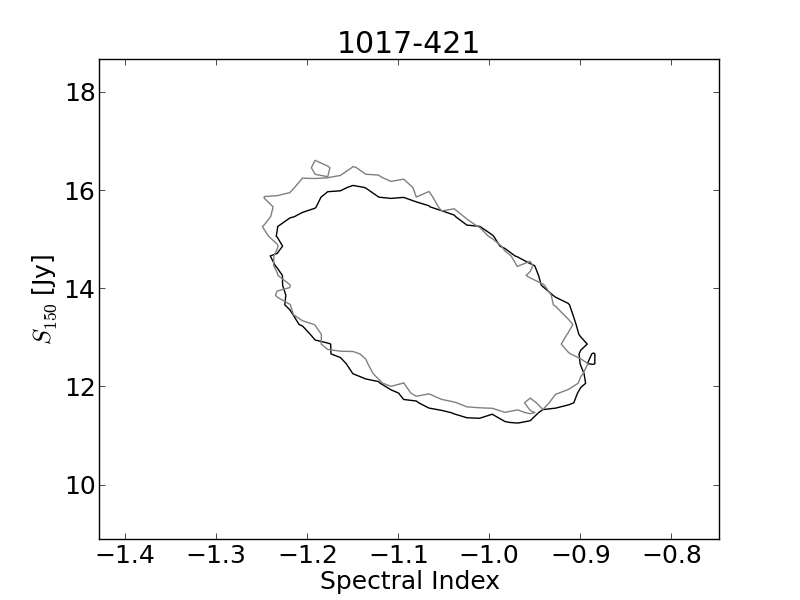
\includegraphics[width=2in]{plots/1017-421_SI_MCMC.png} %0.0034
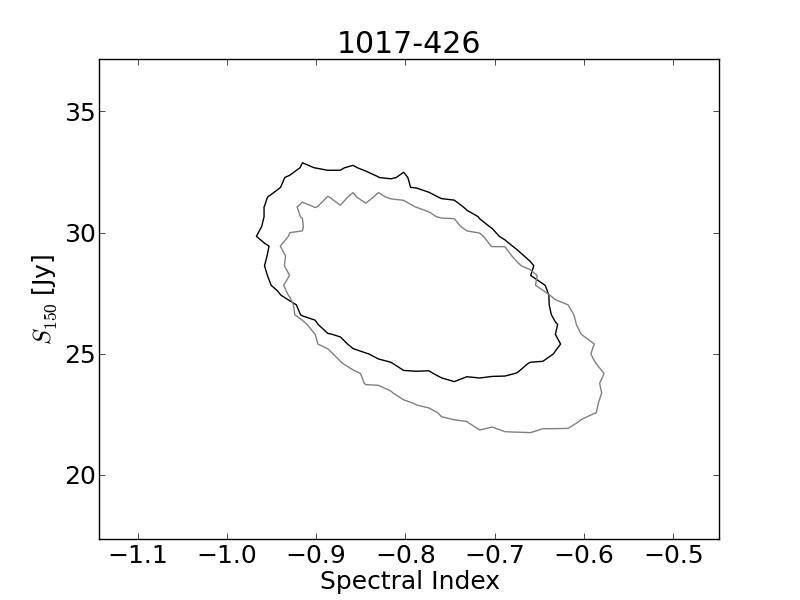
\includegraphics[width=2in]{plots/1017-426_SI_MCMC.png} %0.0195
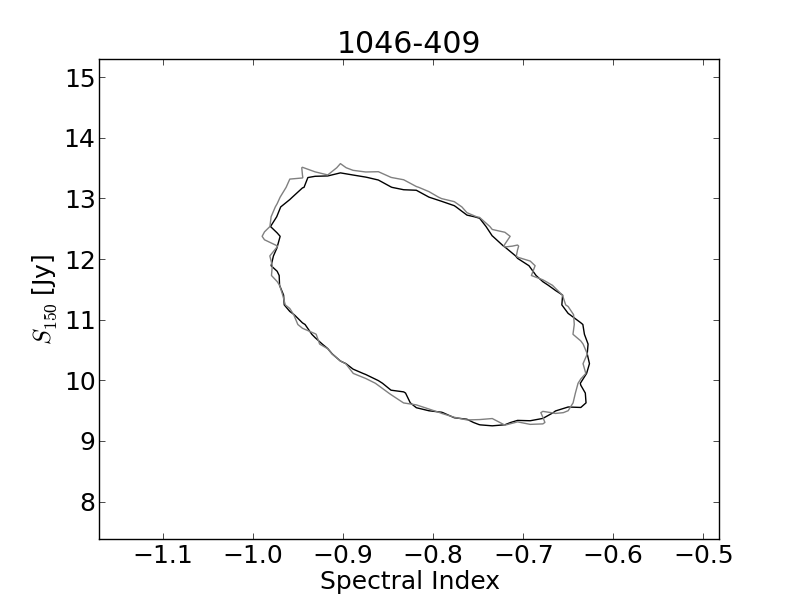
\includegraphics[width=2in]{plots/1046-409_SI_MCMC.png} %0.0012
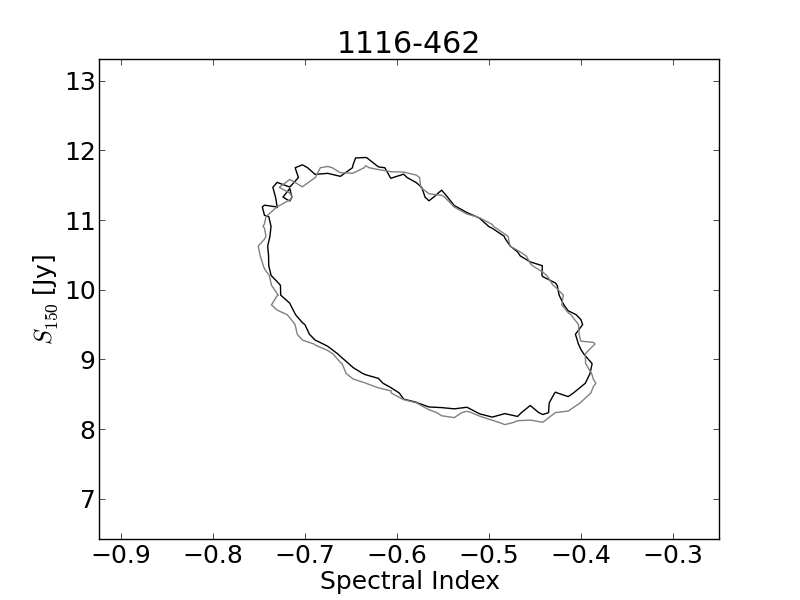
\includegraphics[width=2in]{plots/1116-462_SI_MCMC.png} %0.0062
\end{center}
\caption{Spectral model contours as described in Figure \ref{fig:pic_spectrum}. Sources marked with a
* were used to assess calibration error.
}\label{fig:SI_contour_2}
\end{figure*}
\clearpage
\begin{figure*}[htbp]2\begin{center}
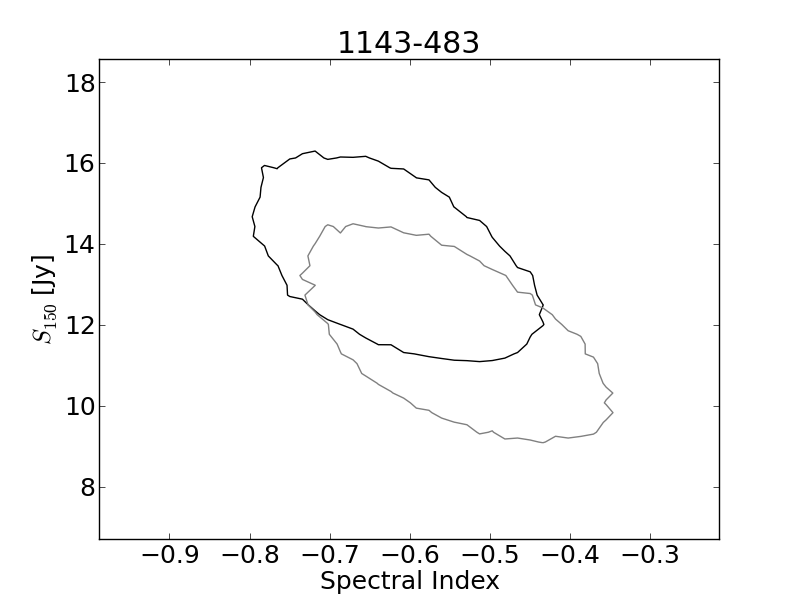
\includegraphics[width=2in]{plots/1143-483_SI_MCMC.png} %0.004
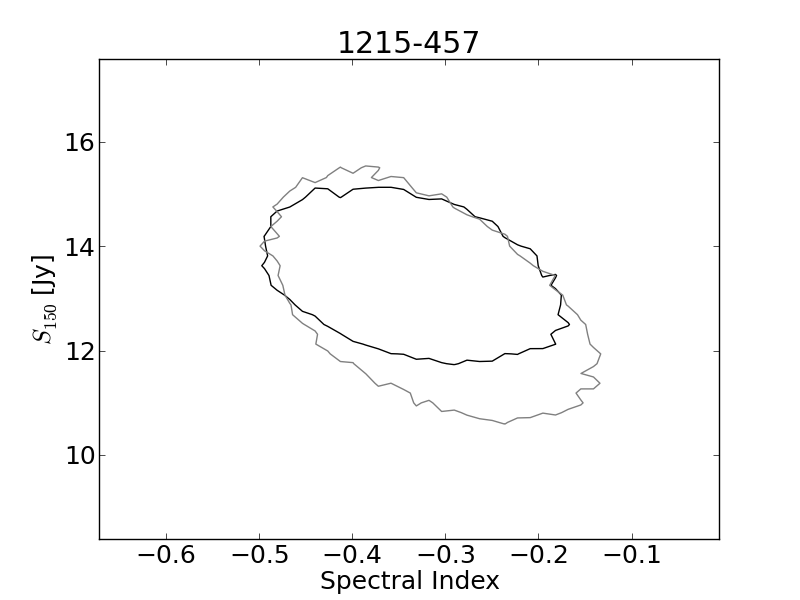
\includegraphics[width=2in]{plots/1215-457_SI_MCMC.png} %0.0163
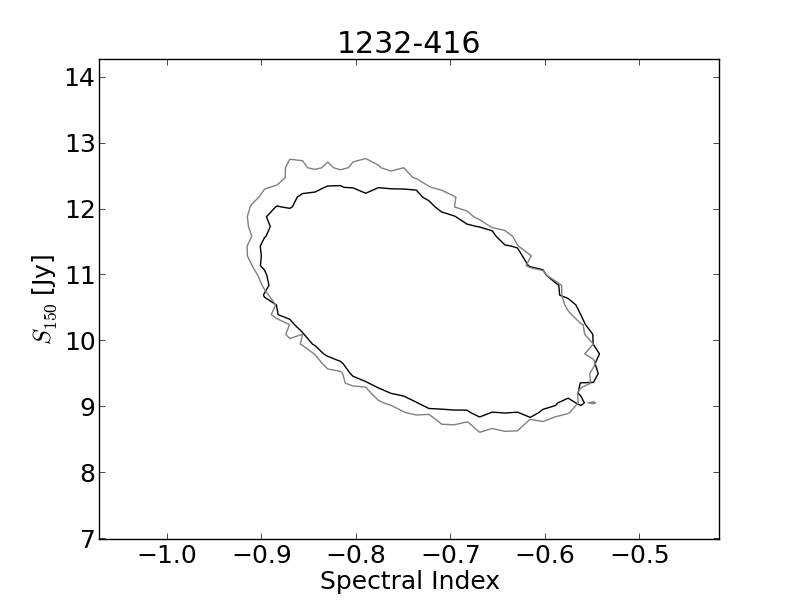
\includegraphics[width=2in]{plots/1232-416_SI_MCMC.png} %0.0227
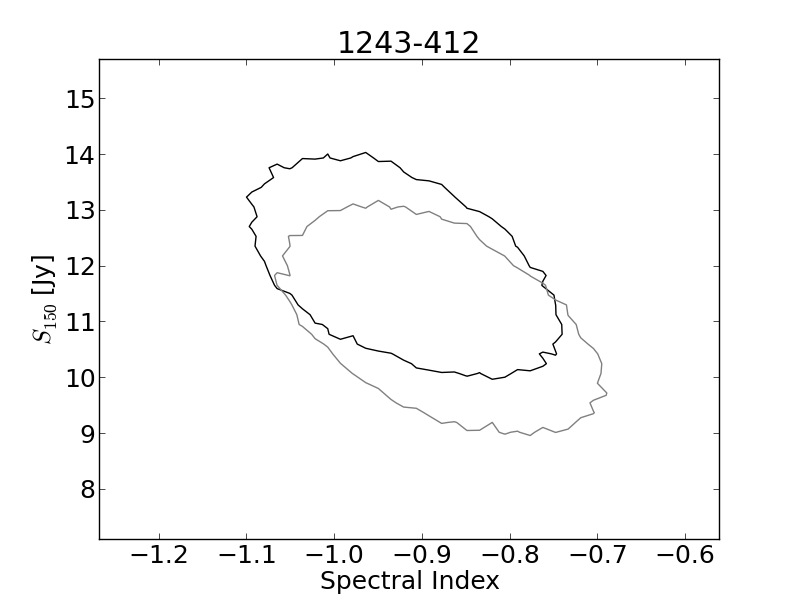
\includegraphics[width=2in]{plots/1243-412_SI_MCMC.png} %0.0076
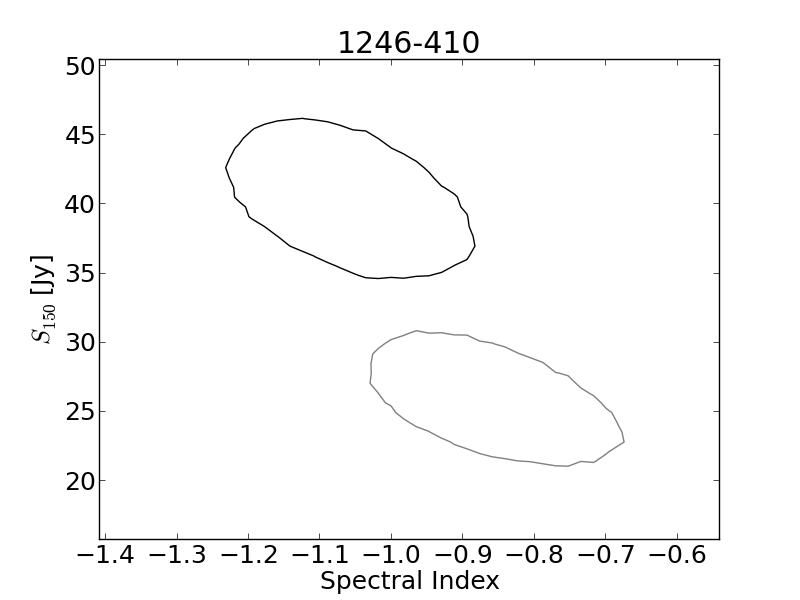
\includegraphics[width=2in]{plots/1246-410_SI_MCMC.png} %0.06
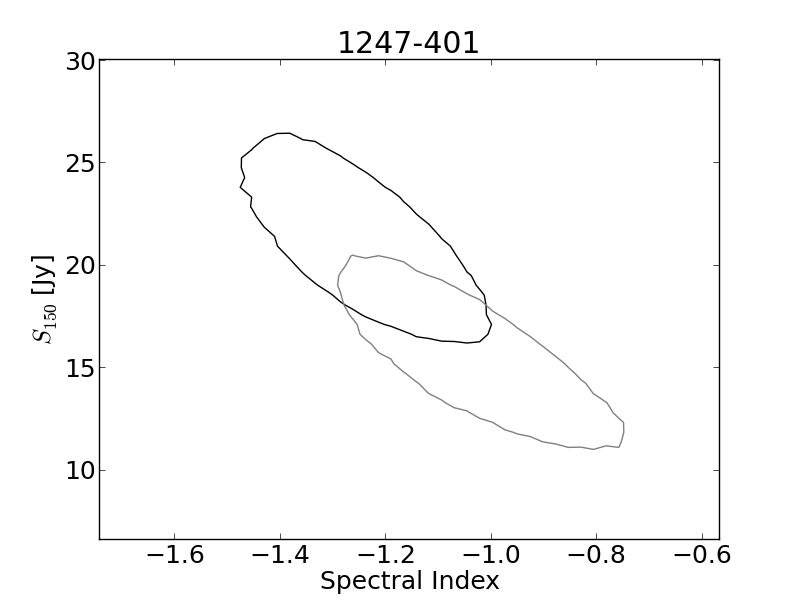
\includegraphics[width=2in]{plots/1247-401_SI_MCMC.png} %0.1161
\includegraphics[width=2in]{plots/1302-491_SI_MCMC.png} %0.5328
\includegraphics[width=2in]{plots/1355-416_SI_MCMC.png} %0.1959
\includegraphics[width=2in]{plots/1358-493_SI_MCMC.png} %0.7284
\includegraphics[width=2in]{plots/1421-490_SI_MCMC.png} %1.3529
\includegraphics[width=2in]{plots/1424-418_SI_MCMC.png} %0.0218
\includegraphics[width=2in]{plots/1445-468_SI_MCMC.png} %1.8104
\end{center}
\caption{Spectral model contours as described in Figure \ref{fig:pic_spectrum}. Sources marked with a
* were used to assess calibration error.
}\label{fig:SI_contour_3}
\end{figure*}
\clearpage
\begin{figure*}[htbp]2\begin{center}
\includegraphics[width=2in]{plots/1526-423_SI_MCMC.png} %0.1985
\includegraphics[width=2in]{plots/1552-433_SI_MCMC.png} %1.3211
\includegraphics[width=2in]{plots/1556-466_SI_MCMC.png} %2.5579
\includegraphics[width=2in]{plots/1616-457_SI_MCMC.png} %0.0507
\includegraphics[width=2in]{plots/1618-430_SI_MCMC.png} %3.821
\includegraphics[width=2in]{plots/1633-409_SI_MCMC.png} %1.3843
\includegraphics[width=2in]{plots/1839-487_SI_MCMC.png} %0.1766
\includegraphics[width=2in]{plots/1840-404_SI_MCMC.png} %0.1658
\includegraphics[width=2in]{plots/1932-464_SI_MCMC.png} %0.4321
\includegraphics[width=2in]{plots/1940-406_SI_MCMC.png} %0.0325
\includegraphics[width=2in]{plots/1953-425_SI_MCMC.png} %0.1181
\includegraphics[width=2in]{plots/2140-434_SI_MCMC.png} %0.2976
\end{center}
\caption{Spectral model contours as described in Figure \ref{fig:pic_spectrum}. Sources marked with a
* were used to assess calibration error.
}\label{fig:SI_contour_4}
\end{figure*}
\clearpage
\begin{figure*}[htbp]2\begin{center}
\includegraphics[width=2in]{plots/2213-456_SI_MCMC.png} %0.2146
\includegraphics[width=2in]{plots/2226-411_SI_MCMC.png} %0.3157
\includegraphics[width=2in]{plots/2250-412_SI_MCMC.png} %0.5585
\includegraphics[width=2in]{plots/2323-407_SI_MCMC.png} %4.9008
\includegraphics[width=2in]{plots/2331-416_SI_MCMC.png} %0.8134
\end{center}
\caption{fits of the last 5 sources, as described in Figure \ref{fig:SI_contour_1}. Sources marked with a
* were used to assess calibration error.
}\label{fig:SI_contour_5}
\end{figure*}%BOTTOM OF MAIN CONFIDENCE PLOT SECTION
%%%%%%%%%%%%%%%%%%%%


%BEGIN PASTE
\begin{figure*}[htbp]
\begin{center}
%ok fit, but doesn't agree with past data, or actually increases model uncertainty
%contour length limit =  223.105907705
%Poor improvement:  1407-425 14.03,15.48,16.92 -1.23,-1.11,-0.99 9.88,11.36,12.93 -1.08,-0.95,-0.82 0.4 0.41 -0.01 0.07 -0.0006 118.0
\includegraphics[width=2in]{plots/1407-425_SI_MCMC.png} %-0.0006
\caption{Contours of spectral fit as described in Figure \ref{fig:SI_contour_1}. This source displays negative 
improvement. The addition of the PAPER data actually slightly increases the uncertainty.
\label{fig:SI_contour_bad}}
\end{center}
\end{figure*}

\begin{figure*}[htbp]
\begin{center}
%zero overlap
\includegraphics[width=2in]{plots/1221-423_SI_MCMC.png} %0.0
\includegraphics[width=2in]{plots/1315-460_SI_MCMC.png} %0.0
\includegraphics[width=2in]{plots/1320-446_SI_MCMC.png} %0.0
\includegraphics[width=2in]{plots/1416-493_SI_MCMC.png} %0.0
\includegraphics[width=2in]{plots/1459-417_SI_MCMC.png} %0
\includegraphics[width=2in]{plots/cen_SI_MCMC.png} %0.0
\end{center}
\caption{
These sources are at odds with previous measurements.
Two simply do not have enough
prior catalog data to fit a spectral model, while the rest have
suggest a deviation from the catalog spectral index fit.
All are near Centaurus A (see Figure
\ref{fig:error_map}), a very bright, extended source, as well as the galactic plane.
Side lobes manifest as
ripples in the beam formed spectra which increases the error bars. See for example the 
Pictor A spectrum \ref{fig:pic_spectrum_detail}. However, the sources shown here are close
enough to Centaurus A that the side-lobe oscillates on scales longer than 10MHz
and does not fall into the rms, but rather into the mean. Thus these few points
have anomalously high fluxes and small error bars. 
} \label{fig:SI_contour_new}
\end{figure*}


%END PASTE



\begin{figure*}
\includegraphics[width=\textwidth]{plots/psa64_pic_strip_positions_annotated_cropped.pdf}
\caption{
A map of the radio sky centered on the south pole
\citep{deOliveiraCosta:2008p2242}.  x's mark measured locations and have size
scaled by dis-agreement with prior data (inverse ``improvement index" from 
\S\ref{sec:fits}). Smaller indicates better agreement with past data.  Black dots indicate sources with $\le0$ improvement score;
agreement decreases with addition of PAPER data (see Figures \ref{fig:SI_contour_bad} and \ref{fig:SI_contour_new}). 
This is most likely due to galactic, and Centaurus A, side lobes.    \label{fig:error_map}
}
\end{figure*}


%TODO catalog format, table for data points and a table for fit results


\begin{deluxetable}{lllllllllllll}
\tablecolumns{13}
\tablecaption{PAPER spectra for 59 MRC sources. Full table available online}
\tablehead{
\colhead{Name} &
\colhead{\parbox[c][3em]{2em}{Ra \unit{deg}}} & 
\colhead{\parbox[c][2em]{2em}{Dec \unit{deg}}} &
\colhead{\parbox[c][2em]{2em}{S125 \unit{Jy}}} &
\colhead{\parbox[c][2em]{2em}{rms \unit{Jy}}} &
\colhead{\parbox[c][2em]{2em}{S135 \unit{Jy}}} &
\colhead{\parbox[c][2em]{2em}{rms \unit{Jy}}} &
\colhead{\parbox[c][2em]{2em}{S145 \unit{Jy}}} &
\colhead{\parbox[c][2em]{2em}{rms \unit{Jy}}} &
\colhead{\parbox[c][2em]{2em}{S155 \unit{Jy}}} &
\colhead{\parbox[c][2em]{2em}{rms \unit{Jy}}} &
\colhead{\parbox[c][2em]{2em}{S165 \unit{Jy}}} &
\colhead{\parbox[c][2em]{2em}{rms \unit{Jy}}}
}
\startdata
Pictor A&	80.1&	-45.79&	459.23&	30.2&	416.59&	28.3&	397.17&	21.8&	375.14&	18.5&	359.72&	17.1 \\
0003-428&	1.67&	-42.5&	14.98&	2.0&	13.45&	1.2&	13.02&	1.8&	12.9&	1.6&	10.42&	1.2 \\
0007-446&	2.79&	-44.31&	23.51&	2.5&	21.18&	2.4&	20.24&	1.5&	18.74&	1.5&	17.61&	1.8 \\
0008-421&	2.88&	-41.81&	-0.94&	1.7&	-0.68&	1.7&	0.54&	1.8&	0.52&	1.4&	1.98&	1.8 \\
0039-445&	10.69&	-44.16&	31.95&	2.9&	30.29&	3.0&	28.54&	2.1&	26.0&	1.9&	24.06&	1.4 \\
0043-424&	11.72&	-42.05&	51.9&	4.2&	47.43&	3.5&	45.82&	2.6&	42.74&	3.0&	40.68&	2.6 \\
0048-447&	12.86&	-44.41&	17.86&	2.6&	16.02&	2.3&	15.15&	2.5&	14.51&	1.5&	12.51&	1.6 \\
0049-433&	13.21&	-43.03&	23.53&	2.4&	21.0&	1.5&	21.94&	2.4&	20.2&	1.9&	18.85&	2.1 \\
0103-453&	16.48&	-45.02&	35.5&	3.2&	32.61&	3.5&	30.86&	2.4&	28.21&	2.5&	27.2&	1.5 \\
0201-440&	31.05&	-43.77&	16.22&	4.4&	15.02&	1.7&	13.73&	1.7&	12.78&	1.2&	14.07&	1.7 \\
0438-436&	70.17&	-43.53&	8.44&	2.5&	6.26&	1.9&	8.05&	1.6&	5.74&	2.1&	9.0&	1.7 \\

\enddata
\label{tab:data}
\end{deluxetable}


%note: put at top of latex file \newcommand{\unit}[1]{\footnotesize \#1}
\begin{deluxetable}{ccccccccccc}
\tablecolumns{11}
\tablecaption{Spectral fits for 52 MRC sources with and without PAPER.}
\tablehead{
\multicolumn{3}{c}{ }&
\multicolumn{4}{c}{PAPER\tablenotemark{1} + Catalog}&
\multicolumn{4}{c}{Catalog\tablenotemark{2}}\\
\colhead{Name} &
\colhead{\parbox[c][3em]{2em}{Ra\\ \unit{deg}}}& 
\colhead{\parbox[c][3em]{2em}{Dec\\ \unit{deg}}} &
\colhead{\parbox[c][3em]{2em}{$S150$\\ \unit{Jy}}} &
\colhead{\parbox[c][3em]{2em}{$\Delta$S\\ \unit{Jy}}} &
\colhead{\parbox[c][3em]{2em}{$\alpha$\\ \unit{--}}} &
\colhead{\parbox[c][3em]{2em}{$\Delta\alpha$\\ \unit{--}}} &
\colhead{\parbox[c][3em]{2em}{$S150_p$\\ \unit{Jy}}} &
\colhead{\parbox[c][3em]{2em}{$\Delta S_p$\\ \unit{Jy}}} &
\colhead{\parbox[c][3em]{2em}{$\alpha_p$\\ \unit{--}}} &
\colhead{\parbox[c][3em]{2em}{$\Delta\alpha_p$\\ \unit{--}}}
}
\startdata
Pictor A&	80.09&	-45.79&	388.92&	9.35&	-0.77&	0.02&	392.08&	21.36&	-0.77&	0.04 \\
0003-428&	1.67&	-42.5&	11.61&	0.54&	-0.81&	0.03&	10.32&	0.76&	-0.73&	0.05 \\
0007-446&	2.79&	-44.31&	18.74&	0.69&	-1.0&	0.03&	16.98&	1.26&	-0.93&	0.05 \\
0039-445&	10.69&	-44.16&	26.77&	1.08&	-0.92&	0.11&	22.71&	5.1&	-0.79&	0.19 \\
0043-424&	11.72&	-42.05&	43.6&	1.46&	-0.79&	0.11&	36.16&	4.97&	-0.69&	0.13 \\
0048-447&	12.86&	-44.41&	13.21&	0.64&	-0.98&	0.04&	11.58&	0.88&	-0.89&	0.05 \\
0049-433&	13.21&	-43.03&	20.16&	0.77&	-0.97&	0.03&	20.54&	1.53&	-0.98&	0.05 \\
0103-453&	16.48&	-45.02&	28.9&	1.14&	-1.16&	0.11&	21.76&	2.93&	-1.04&	0.12 \\
0201-440&	31.05&	-43.77&	13.72&	0.9&	-0.71&	0.12&	10.31&	6.54&	-0.51&	0.42 \\
0438-436&	70.17&	-43.53&	8.08&	0.74&	-0.19&	0.09&	8.32&	1.09&	-0.21&	0.1 \\
0511-484&	78.3&	-48.39&	24.92&	1.59&	-1.14&	0.09&	17.3&	10.7&	-0.93&	0.39 

\enddata
\label{tab:fits}
\tablenotetext{1}{Fits for the majority of sources (78\%) that agree with prior measurements are included here. 
The remainder (the 6 sources shown in Figure \ref{fig:SI_contour_new}) are likely contaminated by bright sources and are not included.   Full table available online.}

\tablenotetext{2}{MCMC fits to prior catalog data, before addition of PAPER measurements}
\end{deluxetable}


%\begin{deluxetable}{ccccccccrrr}
%%\begin{tabular}{ccccccccrrr}
%\tablecolumns{12}
%\tablecaption{Spectral fits for models shown in Figures \ref{fig:SI_contour_1} - \ref{fig:SI_contour_4}.
%\tablehead{
%\colhead{Ra} & \colhead{Dec} & \colhead{Name} & \colhead{S150} & 
%\colhead{e_S150} & \colhead{SI} & \colhead{e_SI}
%\startdata
%
%
%\enddata
%\tablecomments{}
%\label{tab:data}
%\end{deluxetable}

\bibliography{library}

\end{document}
